\chapter{毫米波通信系统中多用户快速跟踪问题研究}

\textbf{本章摘要:} 在毫米波无线通信系统中,为了提供更好的通信质量并降低通信时延,需要实时掌握用户精确的位置信息以进行波束对准与波束跟踪。本章研究了在毫米波通信系统中基站如何通过收集到的位置数据对多个用户进行跟踪,并对可利用的计算资源进行优化管理以提高整个过程的实时性。提出改进的重采样算法,得到一个针对多目标跟踪场景的完全流水线完全并行化概率假设密度(PHD)粒子滤波算法,同时提出了针对多核处理器平台的改进PHD粒子滤波算法及其硬件结构。为了提高多目标跟踪的实时性,建立了最小化总运行时延的优化问题并得到了高效的解法。仿真结果表明,相较于传统PHD粒子滤波算法,提出的完全流水线完全并行化PHD粒子滤波算法大大降低了系统的运行时延,同时保持着相近的跟踪效果。即通过引入改进的重采样算法,提出的优化后算法能够显著提高多目标跟踪的实时性,进而可以降低毫米波无线通信中用户终端的波束对准与跟踪等过程的时延。

\textbf{关键词:}多目标跟踪;实时性;整数规划
%\keywords{多目标跟踪;实时性;整数规划}

\section{引言}

在毫米波无线通信研究中,用户的位置信息至关重要。与传统全向通信模式不同,毫米波信号在空间中极易衰减,需要通过方向性窄波束集中无线信号能量进行传输,这就需要发射与接收端波束互相对准才能建立链接。而只有知道用户的精确位置信息,基站才能够更快地做好毫米波波束对准与跟踪,进而提供更好的通信质量。一个基站下可能有众多的用户需要通信,这就需要同时知道这些用户的精确位置。同时,用户通常不会固定在一个位置,而是在一定范围移动,具有一定的移动性,这就带来了多目标跟踪问题(Multiple Target Tracking, MTT)。

多目标跟踪问题在近些年一直是研究热点,无论是在军事还是民用领域都占有重要的地位。其主要目的是根据一定的观测方式与手段得到观测区域内的目标数量及其各自的状态。多目标跟踪问题主要有两类解决思路,即数据匹配与非数据匹配方法。数据匹配方法是指在定位与跟踪过程中,每次采样得到的用户位置信息要与之前每个用户的航迹信息进行匹配,判断每个样本来自于哪个用户,再进行滤波处理。而非数据匹配方法则不需要采样点与用户航迹的匹配,相较于前者避免了匹配的过程,尤其是在用户数量提高的时候,可以大幅减少计算时间。一般来说,非数据匹配方法主要是指基于随机有限集(Random Finite Sets, RFS)理论的概率假设密度(Probability Hypothesis Density, PHD) 滤波算法。其主要有两种实现形式,一是高斯混合(Gaussian Mixture PHD, GM-PHD)滤波\cite{vo2006gaussian,clark2007convergence},另一种是基于序贯蒙特卡洛\cite{vo2003sequential}(Sequential Monte Carlo, SMC)的粒子滤波(Particle Filter PHD, PF-PHD)形式。两者相较而言,PF-PHD能够更好地处理非线性非高斯的情况,因此更加受到研究者的关注。
多目标跟踪问题的研究难点主要体现在

\begin{enumerate}
  \item 目标数量未知,存在目标的出生、消失、衍生或合并等情况。特别的,在通信领域,主要难点在于对于某一特定的小区(即监测区域内),用户会在任意时刻从邻近小区进入或离开本小区,或在本小区内突然开始通信或停止通信,这就带来了跟踪目标出生与消失的情况。
  \item 监测背景的复杂性,由于存在着杂波、噪声等情况,会降低目标跟踪的精度,并会带来虚警、误警等情况。特别的,在毫米波通信范围内,空间中本身存在的无线电波,或者由目标发出的多径效应产生的信号都会提高背景的复杂度,给准确的目标估计带来困难。
  \item 多目标跟踪的实时性,当目标数量增多,或是要求的精度增高的时候,计算的复杂度就会相应的提高。而无论是在雷达跟踪领域或是民用通信领域,实时性都是影响系统性能的重要指标之一。因此需要不断改进跟踪算法以提高其实时性能。具体而言,更高的实时性意味着更低的通信时延,更短的用户等待时间以及更佳的通信质量。
\end{enumerate}

在多目标跟踪问题中,除了用户的数量和位置信息是否准确以外,跟踪实时性也是一个重要的评价指标。在下一代通信系统中一个重要的挑战就是如何降低通信时延,以提供更快的连接速度。因此,多目标跟踪的实时性就变得更加重要,只有实时地得到多用户的位置信息才能提供更低的通信时延。尽管PHD粒子滤波已经避免了在非线性非高斯情况下的数据匹配问题,其计算复杂度仍然难以满足运算的实时性要求。为了提高运算速率,可以将PHD粒子滤波算法实现在特殊定制的硬件上。一般来说有两类硬件实现平台,一类基于现场可编程门阵列(Field Programmable Gate Array, FPGA)平台\cite{jacobsen2014fpga,hong2011simplified},另一类是基于多核处理器平台\cite{li2016algorithm}。本章主要关注如何在多核处理器平台上建立完全流水线完全并行化多目标跟踪算法,通过对算法步骤的改进与对系统资源的优化分配以降低整个跟踪过程的运行时延。具体而言本章的主要贡献有以下几点:

\begin{enumerate}
	\item 提出了改进的重采样算法,将重采样与预测步骤流水线化,为完全流水线完全并行化PHD粒子滤波算法建立算法基础。
	\item 在多核处理器硬件结构中建立了完全流水线完全并行化PHD粒子滤波算法实现,通过合理分配计算资源以提高滤波过程的实时性。
	\item 依照完成效率不同将滤波算法硬件实现的各种情况进行分类,建立一组混合非线性整数规划问题,并得到其优化解法。仿真结果证明了提出算法有效性与实时性的提高。
\end{enumerate}

本章其余部分组织如下:第2.2节介绍了多目标跟踪领域的研究现状,主要包括PHD滤波算法基础及其实现方法;第2.3节设计了可完全流水线完全并行处理的PHD粒子滤波算法;第2.4节提出了对应的硬件结构优化问题与优化方案;第2.5节仿真结果验证了提出算法的跟踪性能与实时性;最后,第2.6节总结本章并介绍了下一步工作。

\section{研究现状}

\subsection{多目标跟踪算法}
多目标跟踪问题是指在监测区域内同时跟踪多个目标的数量与位置信息。主要有两类算法,一类需要将每次获得的新的观测值与之前得到的航迹信息进行匹配,即数据关联类算法;另一类则不需要两者之间的匹配,即非数据关联算法。数据关联类算法主要包括最近邻匹配算法\cite{singer1971optimal}(NN),多假设跟踪算法\cite{blackman2004multiple}(MHT),联合概率数据关联算法\cite{fortmann1983sonar}(JPDA)等。

\begin{enumerate}

\item{最近邻匹配算法}

最近邻匹配算法需要知道观测场景中目标的数量,其核心是每当新的观测值到达后,找到与每个已有航迹距离最近或者与已有观测似然值最大的点作为其航迹的延续,因此只有那些处于已有航迹附近的新的观测值会延续下去,其余没有对应的观测值则会被记录,当这些观测值能够一直延续三四帧后,则启动一条新的航迹。相较于传统最近邻匹配算法,全局最近邻匹配\cite{sinha2012track}能够保证一个新的观测值只与一个已有航迹进行匹配,而非可以与多个相近的航迹匹配。然而相临近的航迹仍然难以区分新的观测值序列是属于哪个航迹,因此该算法无法处理航迹相近的情况。

\item{多假设跟踪算法}

多假设跟踪算法是利用一组在时间上连续的大概率来源于同一目标的观测值作为航迹的假设,主要分为两类:一类是假设导向的多假设跟踪算法\cite{reid1979algorithm},利用最小均方误差估计-最大后验概率估计(MMSE-MAP);另一类是目航迹导向的多假设跟踪算法\cite{blackman1999design},利用最小均方误差-最大似然估计(MMSE-ML)。航迹会进行聚类 ,同一聚类里的航迹会互相分享假设的观测值,非同一聚类里的航迹则不会分享假设的观测值。每个时刻,多假设跟踪算法会利用上一时刻的航迹假设进行预测,并建立阈值门,每个落在阈值门里的观测值会建立一个关联航迹假设。当一个已有的航迹没有任何一个观测值落在其阈值门内时,则会触发观测丢失事件。不处于任何一个已有航迹的阈值门内的观测值会触发新的航迹。以上两类算法都有着共同的问题,即当假设数量上升时,算法的计算复杂度会指数提升。

\item{联合概率数据关联算法}

联合概率数据关联算法,是基于概率数据关联(PDA)\cite{bar1975tracking}的次优估计算法。PDA算法对所有在确认门中的备选观测值计算其后验联合概率,将其加权和通过卡尔曼滤波(线性模型)或扩展卡尔曼滤波(非线性模型)更新目标状态。联合概率数据关联算法虽然也利用了和PDA相同的估计方法,但是在计算观测值的后验概率时,PDA算法对于每个观测值都分别计算其来自于每个观测目标的后验概率;而JPDA算法则在整个观测目标和杂波集合上进行后验概率的联合计算。在此基础上又有人提出了一些改进方案,如集成概率数据关联算法(IPDA)\cite{musicki1994integrated},其改进版本联合集成概率数据关联算法(JIPDA)\cite{musicki2004joint}以及ML-PDA\cite{kirubarajan1995low,jauffret1990track}等算法。
\end{enumerate}

此外,最近也有文章利用递归神经网络(Recurrent Neural Networks, RNN)来研究多目标跟踪问题\cite{milan2017online}。文章利用递归神经网络实现了对跟踪目标的无模型预测,解决了多目标跟踪领域的先验模型缺失的问题,并且同时可以针对线性与非线性以至于高阶的运动模型。此外,RNN还可以用来解决在目标出生和死亡时整体目标集合数量变化的问题。

以上几种算法有着一个共同的特点,就是需要进行新到观测与已有航迹的匹配。这在目标数量不高的时候是一种有效的跟踪手段。然而随着应用场景与要求的提高,跟踪监测区域内的目标数量越来越多,此时基于数据匹配的算法的计算复杂度就会显著地上升,导致算法性能和实时性的降低。因此有学者提出一些基于非数据匹配的方法。其中最主要的是概率假设密度滤波算法。


\subsection{概率假设密度滤波}

概率假设密度滤波算法是主要基于Mahler提出的有限集统计(Finite Set Statistics, FISST)理论\cite{mahler2007statistical},以贝叶斯滤波作为基础,通过随机有限集理论对复杂观测区域内多个目标进行整体建模,利用随机集的形式表征多目标的状态,其中集合势即元素的个数为目标个数。相较于MHT等滤波算法,PHD滤波算法是一种在计算上更加简单的最优多目标滤波算法,其同时考虑了目标的产生、转移、衍生和消失等情况,避免了观测值与目标轨迹之间的关联,可以直接得到多个目标的数量和位置。 最优贝叶斯多目标滤波的目的是即时的产生多目标的后验概率分布。由于后验概率分布难以得到,只能通过其统计矩来对后验概率分布进行近似。假设使用泊松点过程来表示,则多目标滤波的性质可以通过其一阶矩来表示。

\subsubsection{随机有限集理论}

与单目标跟踪问题不同,多目标跟踪问题中存在着目标生成与消失等情况,其目标状态与测量值的维度随时可能发生变化。一般将$k$时刻的目标状态和测量值分别定义为$X_k$和$Z_k$。$X_k = \{x_{k,1},...,x_{k,M(k)}\} \equiv E_s$代表$k$时刻目标状态空间$E_s$内有$M(k)$个目标的状态信息。$Z_k = \{z_{k,1},...,z_{k,N(k)}\} \equiv E_o$代表$k$时刻观测状态空间$E_o$内有$N(k)$个目标的状态信息。其中$M_k$不等于$N_k$的原因可能来自于目标误报、漏报以及杂波等。

若上一时刻的多目标状态为$X_{k-1}$,则$k$时刻的多目标状态随机有限集\cite{mahler2007phd}表示如下

\begin{equation}
\Xi_k = S_k(X_{k-1})\cup B_k(X_{k-1}) \cup \Gamma_k,
\end{equation}
其中$S_k(X_{k-1})$代表$k$时刻仍然存活的多目标随机有限集,$B_k(X_{k-1})$代表从上一时刻目标中衍生出的目标随机有限集,$\Gamma_k$代表$k$时刻随机生成的目标随机有限集。
可以通过马尔可夫性的条件概率“密度”$f_{k|k-1}(X_k|X_{k-1})$来表征随机有限集$\Xi_k$的统计学特性。

类似地,当给定多目标的状态为$X_k$时,多目标观测值的随机有限集可以表示为
\begin{equation}
\Sigma_k = E_k(X_k) \cup C_k(X_k),
\end{equation}
其中$E_k(X_k)$是从目标生成的观测值随机有限集,$C_k(X_k)$代表杂波或者误警生成的观测值随机有限集。可以通过似然函数形式的条件概率“密度”$ g_k(Z_k|X_k)$来表征随机有限集$\Sigma_k$的统计学特性。

因此,最优多目标贝叶斯滤波算法可以分解为以下迭代步骤,即预测(如图(\ref{PHD}))和更新(如图(\ref{PHDD}))进行
\begin{equation}\label{PHD}
  p_{k|k-1}(X_k|Z_{0:k-1}) = \int f_{k|k-1}(X_k|X)p_{k-1|k-1}(X|Z_{0:k-1}) \mu_s(\mathrm{d}X),
\end{equation}

\begin{equation}\label{PHDD}
p_{k|k}(X_k|Z_{0:k}) = \frac{g_k(Z_k|K_k)p_{k|k-1}(X_k|Z_{0:k-1})}{\int g_k(Z_k|X)p_{k|k-1}(X|Z_{0:k-1}) \mu_s(\mathrm{d}X)},
\end{equation}
其中$p_{k|k}(X_k|Z_{0:k})$是多目标后验“密度”。

概率假设密度$D_{\Xi}$是随机有限集$\Xi$的一阶矩,定义为

\begin{equation}\label{Eq:phd}
  D_{\Xi}(x) \equiv \mathbb{E}[\delta_{\Xi}(x)]=\int \delta_{X}(x)P_{\Xi}(\mathrm{d}X),
\end{equation}
其中$\delta_{Xi}(x)$是随机有限集$\Xi$的随机密度表示,与其以$x\in \Xi$中的每个$x$为中心的狄拉克delta函数的总和相同,
即$\delta_{\Xi}(x) = \sum_{x \in \Xi} \delta_x$。

随机有限集$\Xi$的概率假设密度$D_{\Xi}$在空间$\mathbf{E}$上是唯一的,每个单独的目标存在且其在可测量子集$S\subseteq E$上的积分$\int_{S}D_{\Xi}(x)\lambda(\mathrm{d}x)$可以得到期望的$\Xi$中的元素个数。此外概率假设密度$D_{\Xi}$的峰值为随机有限集$\Xi$中元素的估计值所在。

概率假设密度(PHD)滤波算法主要包括两个操作,预测和更新。假设随机有限集服从泊松分布,则多目标后验概率$p_{k|k}$得概率假设密度$D_{k|k}$的递归生成式为
\begin{equation}\label{Eq:PHD01}
  D_{k|k} = (\Psi_k \circ \Phi_{k|k-1})(D_{k-1|k-1}),
\end{equation}
其中$\Phi_{k|k-1}$是预测操作算子,$\Psi_k$是更新操作算子。它们分别定义如下:

\begin{equation}\label{Eq:PHD02}
  (\Phi_{k|k-1}\alpha)(x) = \int \phi_{k|k-1}(x,\xi)\alpha(\xi)\lambda(\mathrm{d}\xi)+\gamma_k(x),
\end{equation}
\begin{equation}\label{Eq:PHD03}
  (\Psi_k \alpha) = [v(x) + \sum_{z\in Z_k}\frac{\psi_{k,z}(x)}{\kappa_k(z)+\langle \psi_{k,z},\alpha\rangle}]\alpha(x),
\end{equation}
对于在$E_s$上任意的可积方程$\alpha$,其中
\begin{align}\label{Eq:PHD04}
  \phi_{k|k-1}(x,\xi) &= e_{k|k-1}(\xi)f_{k|k-1}(x|\xi)+b_{k|k-1}(\cdot|\xi),\\
  v(x) &= 1-p_D(x),\\
  \psi_{k,z}(x) &= p_D(x)g_k(z|x),\\
  \kappa_k(z) &= \lambda_kc_k(z),
\end{align}
其中$\gamma_k$代表自由生成的目标的随机有限集$\Gamma$的概率假设密度。$b_{k|k-1}(\cdot|\xi)$代表上一时刻状态为$\xi$的衍生目标的随机有限集$B_{k|k-1}(\{\xi\})$的概率假设密度。$e_{k|k-1}(\{\xi\})$代表上一时刻状态为$\xi$的目标在时刻$k$仍然存活的概率。$f_{k|k-1}(\cdot |\cdot)$代表每个目标的状态转移概率。$g_k(\cdot |\cdot)$ 是每个目标的似然函数。$c_k$是杂波的概率密度,$\lambda_k$是平均每个时隙下泊松杂波点的数量。$p_D$是目标被发现的概率。

尽管PHD滤波算法在最优多目标滤波问题上已经是相对计算简单的算法,但是由于引入了大量的积分,使得直接计算依然难以进行。由于PHD滤波算法没有显式的表达,一般采用粒子滤波形式或者高斯混合形式进行实现,其中粒子滤波形式能够更好地处理非线性非高斯的模型。

\subsubsection{概率假设密度粒子滤波算法}

PHD粒子滤波算法基于一般的序贯蒙特卡洛\cite{vo2005sequential}(SMC)方法。其核心在于将难以表达的后验分布方程利用大量的随机分布的采样,通过计算采样信息及其权重以模拟此后验分布,这些采样即称为粒子。当粒子数目足够多的时候,其所表现的特性就能够视为等同于原后验分布方程。

假设$k-1$时刻,对于上节中的可积方程$\alpha$,可以用一组带有权重的粒子$\{w_{k-1}^{(i)},x_{k-1}^{(i)}\}_{i=1}^{L_{k-1}}$表示,即
\begin{equation}\label{PF1}
  \alpha_{k-1}(x) = \sum_{i=1}^{L_{k-1}}w_{k-1}^{(i)}\delta_{x_{k-1}^{(i)}}(x),
\end{equation}
则
\begin{equation}\label{PF2}
    (\Phi_{k|k-1}\alpha)(x) = \int \phi_{k|k-1}(x,\xi)\alpha(\xi)\lambda(\mathrm{d}\xi)+\gamma_k(x_k) = \sum_{i=1}^{L_{k-1}}w_{k-1}^{(i)}\xi_k(x_k,x_{k-1}^{(i)})+\gamma_k(x_k).
\end{equation}

为了得到$\Phi_{k|k-1}\alpha$的粒子估计,需要对其做重要性采样。令从提议分布$q_k(\cdot |x_{k-1}^{(i)},Z_k)$中的$L_{k-1}$个采样为$\{x_k^{(i)}\}_{i=1}^{L_{k-1}}$,从另一个提议分布$p_k(\cdot |Z_k)$中的$J_k$个独立同分布采样为$\{x_k^{(i)}\}_{i=L_{k-1}+1}^{L_{k-1}+J_k}$,即
\begin{displaymath}
    x_k^{(i)} \sim \left\{ \begin{array}{ll}
      q_k\left(\cdot |x_{k-1}{(i)} ,Z_k\right), & i = 1,\dots,L_{k-1} \\
      p_k\left(\cdot | Z_k\right) & i = L_{k-1}+1,\dots,L_{k-1}+J_k
    \end{array}\right.
\end{displaymath}

则可以通过两类粒子$\left\{w_{k-1}^{(i)},x_{k-1}^{(i)}\right\}_{i=1}^{L_{k-1}}$到$\left\{w_{k|k-1}^{(i)},x_{k}^{(i)}\right\}_{i=1}^{L_{k-1}+J_k}$的映射来表示预测操作算子$\Phi_{k|k-1}$
\begin{equation}\label{PF4}
  (\Phi_{k|k-1}\alpha_{k-1})(x_k) \equiv \sum_{i=1}^{L_{k-1}+J_k}w_{k|k-1}^{(i)}\delta_{x_k^{(i)}}(x_k).
\end{equation}
其中
\begin{displaymath}
    w_{k|k-1}^{(i)} \sim \left\{ \begin{array}{ll}
      \frac{\phi_k\left(x_k^{(i)},x_{k-1}^{(i)}\right)w_{k-1}{(i)}}{q_k\left (x_k^{(i)} |x_{k-1}^{(i)} ,Z_k\right)}, & i = 1,\dots,L_{k-1} \\
      \frac{\gamma_k\left(x_k^{(i)}\right)}{J_k p_k\left(x_k^{(i)} | Z_k\right)} & i = L_{k-1}+1,\dots,L_{k-1}+J_k
    \end{array}\right.
\end{displaymath}

类似地,更新操作算子$\Psi_k$可以通过两类粒子$\left\{w_{k|k-1}^{(i)},x_{k}^{(i)}\right\}_{i=1}^{L_{k-1}}$到$\left\{w_{k}^{(i)},x_{k}^{(i)}\right\}_{i=1}^{L_{k-1}+J_k}$的映射来更新粒子权重
\begin{equation}\label{PF5}
  (\Psi_k \alpha_{k|k-1})(x) =  \sum_{i=1}^{L_{k-1}+J_k}w_{k}^{(i)}\delta_{x_k^{(i)}}(x),
\end{equation}
其中
\begin{align}\label{PF6}
  (w_k^{(i)}) & = [v(x^{(i)}) + \sum_{z\in Z_k}\frac{\psi_{k,z}(x)}{\kappa_k(z)+C_k(z)}]w_{k|k-1}^{(i)},\\
  C_k(z) & = \sum_{j=1}^{L_{k-1}+J_k}\psi_{k,z}(x_{k}^{(j)})w_{k|k-1}^{(j)}.
  \end{align}

在预测和更新的循环之外,还需要提取保存在粒子中的目标状态信息\cite{si2016multi}。一般通过聚类算法\cite{clark2007multi}将来源于不同目标的粒子进行区分,再从中提取目标的位置信息。通常采用的方法有k均值方法,CLEAN算法\cite{tobias2008techniques}。

此外,有研究提出了势概率假设密度滤波算法\cite{mahler2007phd}(Cardinalized Probability Hypothesis Density, CPHD)。此类算法在PHD滤波算法的基础上,增加了对集合势分布的迭代,并利用最大后验估计(Maximum a Posteriori, MAP)对多目标的数量进行估计。这种方式提高了滤波算法对目标数量的估计准确度,但同时也带来了更高的计算复杂度。若粒子数目为$N$,观测值数目为$M$,则PHD粒子滤波算法的计算复杂度为$O(NM^2)$,而CPHD粒子滤波算法的计算复杂度为$O(NM^2 + M^3)$\cite{nannuru2013computationally}。

\subsubsection{概率假设密度高斯混合滤波算法}

高斯混合实现是利用混合高斯模型来估计随机有限集的后验分布,这建立在目标的先验分布是高斯混合加权和的形式前提下。因此高斯混合PHD算法只适用于运动目标线性高斯的情况。
每个目标都服从一个线性高斯动态模型,观测者则服从一个线性高斯观测模型,即
\begin{equation}
f_{k|k-1}(x|\zeta) = \mathcal N(x;F_{k-1}\zeta,Q_{k-1}),
\end{equation}
\begin{equation}
g_k(z|x) = \mathcal N(z;H_kx,R_k).
\end{equation}
其中$\mathcal N(\cdot;m,P)$代表均值为$m$,方差为$P$的高斯密度分布,$F_{k-1}$代表状态转移矩阵,$Q_{k-1}$是过程噪声协方差;$H_K$是观测矩阵,$R_k$是观测噪声协方差。

目标的存活概率和检测概率与状态无关,分别为$p_{S,k}(x) = p_{S,k}$和$p_{D,k}(x) = p_{D,k}$。
目标的生成强度为
\begin{equation}
\gamma_k(x) = \sum_{i=1}^{J_{\gamma,k}}w_{\gamma,k}^{(i)}\mathcal N(x;m_{\gamma,k}^{(i)},P_{\gamma,k}^{(i)}).
\end{equation}
目标的衍生概率为
\begin{equation}
\beta_{k|k-1}(x|\zeta) = \sum_{j=1}^{J_{\beta,k}}w_{\beta,k}^{(j)}\mathcal N(x; F_{\beta,k-1}^{(j)}\zeta+d_{\beta,k-1}^{(j)},Q_{\beta,k-1}^{(j)}).
\end{equation}
其中$J_{\gamma,k}$, $w_{\gamma,k}^{(i)}$,$m_{\gamma,k}^{(i)}$,$P_{\gamma,k}^{(i)},i = 1,\dots,J_{\gamma,k}$是给定的决定生成强度形状的模型参数;类似地,
$J_{\beta,k}$, $w_{\beta,k}^{(i)}$, $F_{\beta,k-1}^{(i)}$, $d_{\beta,k-1}^{(i)}$, $Q_{\beta,k-1}^{(i)}$决定了上一时刻状态为$\zeta$的目标衍生强度的形状。

在此基础上,$k-1$时刻后验强度的高斯混合表达形式为
\begin{equation}
v_{k-1}(x) = \sum_{i=1}^{J_{k-1}}w_{k-1}^{(i)}\mathcal N(x;m_{k-1}^{(i)},P_{k-1}^{(i)}).
\end{equation}
$k$时刻的预测强度为
\begin{equation}
v_{k|k-1}(x) = v_{S,k|k-1}(x) +v_{\beta,k|k-1}(x)+ \gamma_k(x).
\end{equation}
得到从$v_{k-1}$计算预测$v_{k|k-1}$的均值、方差和权重的封闭解表达式。
$k$时刻预测强度的高斯混合表达形式为
\begin{equation}
v_{k|k-1}(x) = \sum_{i=1}^{J_{k|k-1}}w_{k|k-1}^{(i)}\mathcal N(x;m_{k|k-1}^{(i)},P_{k|k-1}^{(i)}),
\end{equation}
$k$时刻的后验强度的高斯混合表达形式为
\begin{equation}
v_k(x) = (1-P_{D,k})v_{k|k-1}(x) + \sum_{z\in Z_k}v_{D,k}(x,z).
\end{equation}
其中
\begin{align}
v_{D,k}(x;z) &= \sum_{j=1}^{J_{k|k-1}}w_{k}^{(j)}(z)\mathcal N(x;m_{k|k}^{(j)}(z),P_{k|k}^{(j)}),\\
w_k^{(j)}(z) &= \frac{p_{D,k}w_{k|k-1}^{(j)}q_k^{(j)}(z)}{\kappa_k(z)+p_{D,k}\sum_{l=1}^{J_{k|k-1}}w_{k|k-1}^{(l)}q_k^{(l)}(z)},\\
m_{k|k}^{(j)}(z) &= m_{k|k-1}^{(j)} + K_k^{(j)}(z- H_km_{k|k-1}^{(j)}),\\
P_{k|k}^{(j)} &= [I - K_k^{(j)}H_k]P_{k|k-1}^{(j)},\\
K_k^{(j)} &= P_{k|k-1}^{(j)}H_k^T(H_kP_{k|k-1}^{(j)}H_k^T+R_k)^{-1}.
\end{align}

在得到了新的观测值之后,从$v_{k|k-1}$计算更新值$v_{k}$的均值、方差和权重的封闭解表达式。
借由以上预测和更新步骤,即可以得到基于高斯混合形式的PHD滤波算法。在最终的目标估计时,也不需要PHD粒子滤波算法中的聚类算法等来提取目标信息,只需提取权重大于某一阈值的高斯分量的均值即可。

\subsubsection{多目标多伯努利滤波算法}

在PHD滤波算法后,Mahler又提出了多目标多伯努利滤波算法(Multi-Target Multi-Bernoulli Filter, MeMBer Filter)\cite{mahler2007statistical}。PHD滤波算法的迭代过程主要是针对随机有限集的一阶矩和势。而多目标多伯努利算法则是迭代的多目标后验概率密度。对于多目标贝叶斯滤波算法来说,最主要的难点在于预测集合和贝叶斯更新的集合积分难以有闭式的表达式。对于卡尔曼滤波算法而言,由于所有相关的分布,包括似然函数,马尔科夫密度,后验密度等都具有线性高斯的特性,因此对于单目标贝叶斯滤波算法而言,卡尔曼滤波能够得到很好的闭式解。而对于多目标的贝叶斯跟踪滤波,当其相关的分布都具有一定特征时,也就是都符合多伯努利过程时,也可以得到闭式的解。相对于SMC-PHD滤波算法的目标估计只能通过聚类等方法得到,BT Vo等人提出的CBMeMBer\cite{vo2009cardinality}算法可以更加简单地进行目标的估计。

对于伯努利随机有限集而言,以概率$1-r$为一个空集,概率$r$为一个单元素集,其在状态空间上的分布为$p(\cdot)$。其势分布服从伯努利分布,概率密度服从
\begin{equation}
   \pi(x) =  \left\{ \begin{array}{ll}
   1-r & X = \emptyset,\\
   r \cdot p(x) &X = \{x\}.
    \end{array}\right.
\end{equation}
而多目标伯努利随机有限集就是由多个互相独立的伯努利有限集的集合。

在进一步的工作中,Reuter等人提出的标签MeMBer滤波算法\cite{reuter2014labeled}。其核心思想是将标签$l$加入到迭代过程中,以便于在多目标跟踪场景中对某一目标的轨迹进行持续性跟踪\cite{vo2013labeled}。

\section{完全流水线完全并行PHD粒子滤波算法}

本文主要研究基于PHD粒子滤波算法的多目标跟踪问题。PHD粒子滤波算法包括四个主要步骤:即预测、更新、重采样和目标估计。对于一个多目标跟踪问题,预测步骤会生成两类粒子,即新生粒子和存活粒子,分别代表新生目标和存活目标的概率分布。更新步骤接收到新的采样观测,并对预测的采样粒子权重进行重新评估。重采样步骤主要用来降低粒子退化现象造成的影响。目标估计步骤用于估计目标的数量及其各自的位置。

在利用粒子滤波方法进行多次迭代计算后会产生粒子退化问题,即粒子权重会集中在某些权值极大的粒子上。这会带来两种情况,一是相当大的计算量会浪费在那些权值很小的粒子上,这些粒子的权重几乎为零,其所消耗的计算能力并不能提升跟踪的效果;二是由于权重的集中,粒子的多样性会严重降低,以至于难以模拟新观测值带来的后验概率变化。因此在PHD粒子滤波算法中,必须引入重采样算法,以减小粒子退化现象造成的影响。

在传统的PHD粒子滤波算法中,重采样操作只有在得到所有粒子的权重值之和后才能进行,这就使得更新和重采样之间的流水线化运算难以进行。为了解决此问题,有学者提出了阈值重采样算法 \cite{shi2013threshold}使得更新与重采样直接可以达到流水线式运算。然而由于重采样过程中的复制运算,此算法仍然不能达到重采样与预测步骤之间的完全流水线化运算。对此本文提出一种改进的重采样算法,用以达到重采样与预测步骤之间的流水线运算,进而得到从更新步骤到预测步骤之间完全流水线化运算。

\begin{figure}[htbp]
\centering
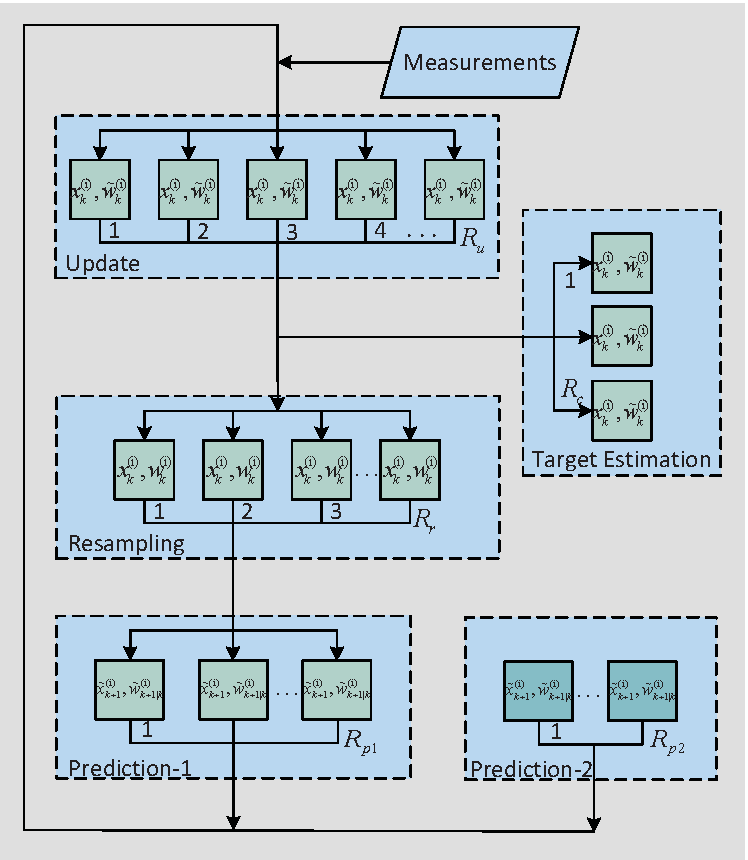
\includegraphics[width=0.9\textwidth]{Pictures/PHD-1.pdf}
\caption{完全流水线完全并行化PHD粒子滤波算法流程示意图}\label{PHD1}
\end{figure}

如图(\ref{PHD1}),参数$R_u$,$R_r$,$R_{p1}$,$R_{p2}$和$R_c$分别表示更新、重采样、存活目标预测(prediction-1)、新生目标预测(prediction-2)以及目标预测等各个步骤的并行运算模块数量。以下将介绍整个完全流水线完全并行PHD粒子滤波算法的运算过程。当然,在整个运算的起始阶段,预测模型会生成起始粒子,每当新的观测结果到达后,整个滤波算法就会运行一个循环。

\textbf{步骤1}:预测

如图(\ref{PHD1}),所有粒子将会按照不同的任务,即存活目标采样和新生目标采样,被平均分配到 $R_{p1}$ 和 $R_{p2}$ 个并行运算单元中。令
$\tilde{\mathbf{x}}_k^{(i)}$ 代表$k$时刻的第$i$个粒子状态,$L$代表存活目标的粒子数量。将 $L$ 个粒子平均分配到 $R_{p1}$ 个存活目标预测单元中, 则每个单元中的粒子数量为 $N_l^{p1} = \underbrace{\lceil\frac{L}{R_{p1}} \rceil,\dots,\lceil\frac{L}{R_{p1}} \rceil}_{mod(L,R_{p1})}$, $\underbrace{\lfloor\frac{L}{R_{p1}} \rfloor,\dots,\lfloor\frac{L}{R_{p1}} \rfloor}_{R_{p1}-mod(L,R_{p1})}, l = 1,\cdots,R_{p1}$,其中 $\lceil\quad\rceil$ 表示向上取整, $\lfloor\quad\rfloor$代表向下取整。$mod(\cdot)$ 代表取模运算。
对每个存活目标预测单元中的粒子$i=1,\cdots,N_l^{p1}$ 从提议分布 $\tilde{\mathbf{x}}_k^{(i)}$ 进行采样
$q_k(\cdot|\mathbf{x}_{k-1}^{(i)},\mathbf{Z}_k)$,其中 $\mathbf{Z}_k$ 是接收到的测量值。
计算存活粒子权重
\begin{equation}\label{Eq:02}
\tilde{w}_{k|k-1}^{(i)}=\frac{\phi_{k|k-1}(\tilde{\mathbf{x}}_k^{(i)},\mathbf{x}_{k-1}^{(i)})}{q_k(\tilde{\mathbf{x}}_k^{(i)}|\mathbf{x}_{k-1}^{(i)},\mathbf{Z}_k)}w_{k-1}^{(i)},
\end{equation}
且
\begin{equation}
\phi_{k|k-1}=e_{k|k-1}f_{k|k-1}+b_{k|k-1},
\end{equation}
其中 $e_{k|k-1}$ 是存活概率, $f_{k|k-1}$是转移概率密度,$b_{k|k-1}$ 是衍生粒子的概率假设密度。

令 $J$ 为新生目标的粒子数量。在$R_{p2}$个新生目标预测单元中平均分配$J$个粒子。则每个单元中的粒子数量为 $N_l^{p2} = \underbrace{\lceil\frac{J}{R_{p2}} \rceil,\dots,\lceil\frac{J}{R_{p2}} \rceil}_{mod(J,R_{p2})},\\ \underbrace{\lfloor\frac{J}{R_{p2}} \rfloor,\dots,\lfloor\frac{J}{R_{p2}} \rfloor}_{R_{p2}-mod(J,R_{p2})}, l = 1,\cdots,R_{p2}$。对于每个单元中的粒子 $i=1,\cdots,N_l^{p}$ ,依照提议分布$
p_k(\cdot|\mathbf{Z}_k)$进行采样 $\tilde{\mathbf{x}}_k^{(i)}$ 。
计算新生粒子权重
\begin{equation}\label{Eq:03}
\tilde{w}_{k|k-1}^{(i)}=\frac{1}{J}\frac{\gamma_k(\tilde{\mathbf{x}}_k^{(i)})}{p_k(\tilde{\mathbf{x}}_k^{(i)}|\mathbf{Z}_k)},
\end{equation}
其中 $\gamma_k$是新生粒子的概率假设密度。

\textbf{步骤2}:更新

所有 $L+J$ 个粒子被平均分配在 $R_{u}$ 个并行的更新单元中,则每个单元中的粒子数目为 $N_l^u = \underbrace{\lceil\frac{L+J}{R_{u}} \rceil,\dots,\lceil\frac{L+J}{R_{u}} \rceil}_{mod(L+J,R_{u})}$, $\underbrace{\lfloor\frac{L+J}{R_{u}} \rfloor,\dots,\lfloor\frac{L+J}{R_{u}} \rfloor}_{R_{u}-mod(L+J,R_{u})}, l=1,\cdots,R_u$. 对于每个新到的观测值$\mathbf{z}\in \mathbf{Z}_k$,计算
\begin{equation}\label{Eq:04}
C_k(\mathbf{z})=\sum_{j=1}^{L+J}\psi_{k,\mathbf{z}}(\tilde{\mathbf{x}}_k^{(j)})\tilde{w}_{k|k-1}^{(j)},
\end{equation}
其中 $\psi_{k,\mathbf{z}}(\mathbf{x})=P_D(\mathbf{x})g_k(\mathbf{z}|\mathbf{x})$, $P_D$ 是发现概率, $g_k(\cdot|\cdot)$是每个目标的似然概率。
对于每个更新单元$l$中的粒子 $i=1,\cdots,N_l^u$ ,更新权重
\begin{equation}\label{Eq:05}
\tilde{w}_k^{(i)}=\left[1-P_D+\sum_{\mathbf{z}\in
\mathbf{Z}_k}\frac{\psi_{k,\mathbf{z}}(\tilde{\mathbf{x}}_k^{(i)})}{\kappa_k(\mathbf{z})+C_k(\mathbf{z})}\right]\tilde{w}_{k|k-1}^{(i)},
\end{equation}
其中 $\kappa_k(\mathbf{z})=\lambda_k c_k(\mathbf{z})$,$\lambda_k$ 是每次搜索中服从泊松分布的杂波的平均数量,$c_k$是杂波概率密度。
继而计算所有粒子的权重和 $S_k=\sum{{\tilde{w}}_k^{(i)}}$。

\textbf{步骤3}: 改进重采样算法

重采样的目的是为了避免粒子退化问题。在大多数重采样算法中,粒子的复制过程需要在所有粒子进行归一化以后才能开始,也就是说在更新步骤中的最后一个粒子完成更新之前,所有的粒子都不能进行复制运算。尽管一些基于阈值的重采样方法能够避免归一化过程,复制过程仍然需要在那些被复制的粒子全部得到后才能进行。 此问题导致了重采样步骤与预测步骤之间流水线化运算难以进行,以致降低整个滤波算法的并行化运算效率。

为了解决此问题,本章提出了一种改进的重采样策略,见算法(\ref{alg:frame})。其核心在于粒子事实上并不需要所有其它粒子的信息才能进行重采样和复制,也就是说,一个粒子可以只在了解自身信息以及在其前的粒子信息就能完成其自身的重采样过程,并不需要在其后的粒子的信息。这样就能够使整个运算达到流水线化运行。


\begin{algorithm}[htbp]

	\caption{改进的重采样算法}\label{alg:frame}
	\SetAlgoLined
	
	\textbf{输入}: $\tilde{\mathbf{x}}_k^{(i)},\tilde{w}_k^{(i)}, i=1,\cdots,N_l^r$, 随机序列 $A$\;
	\textbf{初始化}: $j=1, m=1, F_l=0$\;
	\For{每一个重采样单元$l$中的 $i = 1,\cdots,N_l^r$}
	{
		\eIf{$ \tilde{w}_k^{(i)} < T_h $}
		{
			\eIf{$ F_l == 0 $}
			{
				\If {$i \in A$}
				{
				$\mathbf{x}_k^{(m)} = \tilde{\mathbf{x}}_k^{(i)}$\;
				$m = m+1$\;
				}
			}		
			{
				\If{$i \in A$}
				{
					得到目前最少复制次数$d_{\underline{j}}$的粒子$\mathbf{Temp}_{\underline{j}}$ \;
					$\tilde{\mathbf{x}}_k^{(i)} = \mathbf{Temp}_{\underline{j}}$\;
					$\mathbf{x}_k^{(m)} = \tilde{\mathbf{x}}_k^{(i)}$\;
					$d_{\underline{j}}=d_{\underline{j}}+1$, $m = m+1$\;
				}
	
			}
		}	
		{
			$F_l=1$\;
			$\mathbf{Temp_j}=\tilde{\mathbf{x}}_k^{(i)}$\;
			$d_j=0$, $j = j+1$\;
			\If{$i \in A$}
			{
				$\mathbf{x}_k^{(m)} = \tilde{\mathbf{x}}_k^{(i)}$\;
				$d_j = d_j+1$, $m = m + 1$\;
			}
		}
	}
	\textbf{输出}: $\mathbf{x}_k^{(m)}, m=1,\cdots,M_l^r$, $w_k^{(m)}=S_{k-1}/L, m= 1,\cdots,M_l^r$.\
\end{algorithm}

具体来说,首先建立一个事先定好的随机的\emph{\textbf{粒子复制序列集合}},用以决定哪些粒子能够被复制。此集合的目的是为了保证重采样过后的粒子数目为一个确定的数量。 如图(\ref{PHD2})所示,待复制粒子通过基于阈值的方法\cite{shi2013threshold} 进行选择。当重采样开始后,在第一个待复制粒子出现前,所有粒子都保持不变:如果此粒子在存活序列中,则复制其本身;否则直接抛弃。当第一个待复制粒子出现后,这些待复制粒子的信息将会被存储到等待列表中。如果待复制粒子本身就在存活序列中,则复制其本身。当一个非待复制粒子在存活序列中时,则令他复制等待列表中的当前复制次数最小的那个粒子信息。 对于剩余的不在存活序列中的粒子则直接放弃。经过该过程,绝大部分重要的粒子将会被保存并复制下去。

\begin{figure*}[htbp]
	\centering
	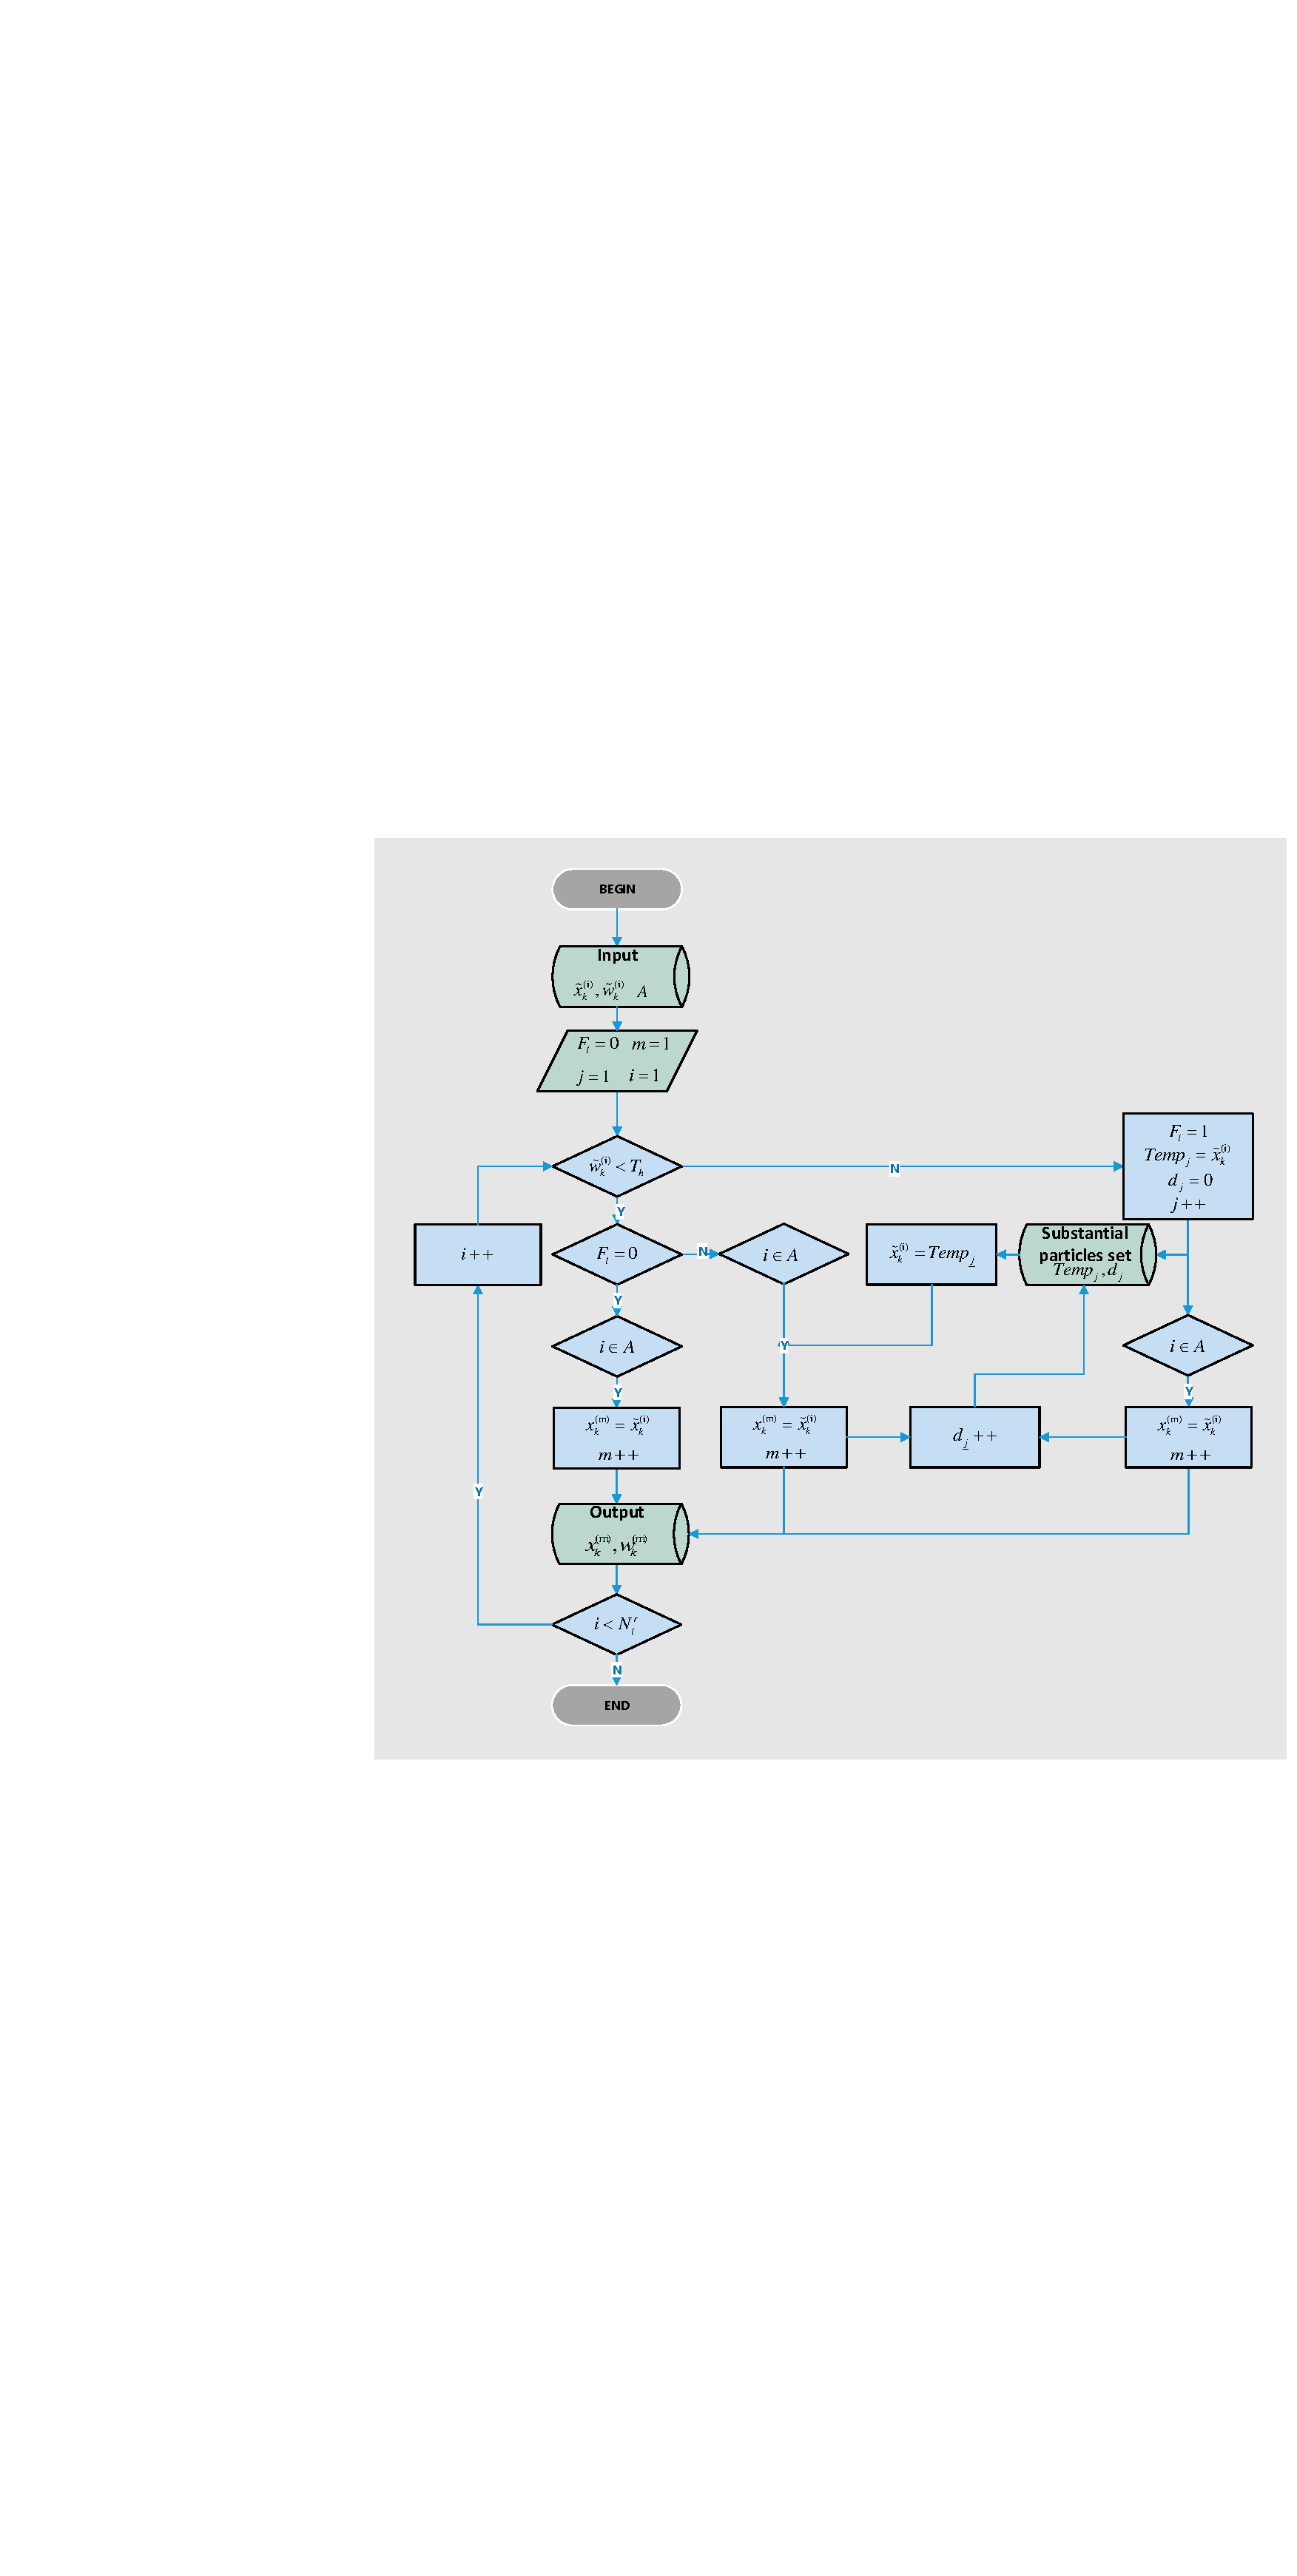
\includegraphics[width=0.9\textwidth]{Pictures/PHD-2.pdf}
	\caption{改进的重采样算法(\ref{alg:frame})流程图}
	\label{PHD2}
\end{figure*}

在此算法中,所有 $L+J$ 个粒子会被平均分配到 $R_{r}$个并行的重采样单元中,则每个重采样单元中的粒子数目为  $N_l^r = \underbrace{\lceil\frac{L+J}{R_{r}} \rceil,\dots,\lceil\frac{L+J}{R_{r}} \rceil}_{mod(L+J,R_{r})}$, $\underbrace{\lfloor\frac{L+J}{R_{r}} \rfloor,\dots,\lfloor\frac{L+J}{R_{r}} \rfloor}_{R_{r}-mod(L+J,R_{r})}, l=1,\cdots,R_r$。重采样后,最终有 $L$ 个粒子存活,每个单元中的粒子数目变为 $M_l^r = \underbrace{\lceil\frac{L}{R_{r}} \rceil,\dots,\lceil\frac{L}{R_{r}} \rceil}_{mod(L,R_{r})}$, \\$\underbrace{\lfloor\frac{L}{R_{r}} \rfloor,\dots,\lfloor\frac{L}{R_{r}} \rfloor}_{R_{r}-mod(L,R_{r})}$。
复制列表$A$的生成方法如下:为了使需要复制的粒子序号随机,将整个按照序号排列的粒子序号打乱,并选取前 $M_l^r$个序号作为存活粒子序号。在之后的重采样过程中,如果粒子序号在该列表中,则会复制一个粒子信息并继续存活下去,否则将会被直接放弃掉。

算法中, $F_l$ 代表是否出现了待复制粒子。
$\mathbf{Temp_j}$ 代表等待序列,,用以暂时储存带复制粒子的序号 $j$和当前已复制次数$d_j$, $\mathbf{x}_k^{(m)}$ 表示从采样的粒子,可以被每个重采样单元读写。最后,在所有粒子运算完成后,粒子 $\{\tilde{w}_k^{(i)},\tilde{\mathbf{x}}_k^{(i)}\}_{i=1}^{L+J}$ 就会被重采样为$\{w_k^{(i)},\mathbf{x}_k^{(i)}\}_{i=1}^{L}$。


\textbf{步骤4}:目标估计

估计目标数量
\begin{equation}\label{Eq:07}
N_k=[S_{k}],
\end{equation}

其中$[\quad]$代表取整运算。每个目标的估计状态可以通过在$R_c$ 个估计模块中,将PHD的后验概率进行聚类得到各个峰值所在点。本章中使用的K-means聚类算法同样可以并行运算\cite{joshi2003parallel}。

\section{硬件资源优化}

在提出完全流水线完全并行化PHD粒子滤波算法的基础上,为了进一步的优化系统资源,提高多目标跟踪的实时性能,需要对运行算法的硬件资源进行优化,合理分配每个算法步骤在多核处理器中所占用的计算资源数量。本章将提出的PHD粒子滤波算法硬件结构资源优化问题建模为一个整数规划问题,并提出一个有界限制的近似解法。

\subsection{优化问题建模}

令 $(T_{p1},S_{p1})$, $(T_{p2},S_{p2})$, $(T_{u},S_u)$, $(T_{r},S_r)$ 和 $(T_{c},S_c)$ 表示存活预测、新生预测、更新、重采样和目标估计的运行时延和资源分配数量。总的可运行资源为$S$,即处理器数量。
%The number of particles is denoted as $L_{k}=Q_1+Q_2$, with $Q_1$ for survival targets and $Q_2$ for newborn targets in the prediction step.
从图(\ref{PHD1})可以发现新生粒子的产生和目标估计是两个独立于迭代循环的模块。同时,这两个模块所消耗的时间都远远小于主迭代循环中存活预测,更新和重采样模块所消耗的时延。因此,总运行时延主要由主循环中的三个模块所决定。所以根据不同的相对运行速率$\begin{aligned}\frac{R_{u}}{T_{u}}\end{aligned}$, $\begin{aligned}\frac{R_{r}}{T_{r}}\end{aligned}$ 和 $\begin{aligned}\frac{R_{p1}}{T_{p1}}\end{aligned}$, 总运行时延的分析与优化过程将主要分成如下四类情况。

\emph{\textbf{情况 $1$}}: $\begin{aligned}\frac{R_u}{T_u}<\frac{R_r}{T_r}<\frac{R_{p1}}{T_{p1}}.\end{aligned}$

当更新模块的相对运行速率最小,其次是重采样模块时,粒子将会首先堵在更新模块,之后会堵在重采样模块。因此总的运行时延可以最小化为

\begin{equation}\label{Eq:08}
\begin{split}
&\min \,\, T=\lceil\frac{L+J}{R_{u}}\rceil T_{u}+\lceil\frac{R_{u}}{R_{r}}\rceil T_{r}+\lceil\frac{L}{L+J}\frac{R_r}{R_{p1}}\rceil T_{p1}\\
&s.t.\quad  \left\{\begin{array}{l}
\begin{aligned}\frac{R_u}{T_u}<\frac{R_r}{T_r}<\frac{R_{p1}}{T_{p1}}\end{aligned} \\
R_{u}<L+J\\
R_{r}<L+J
R_{p1}<L \\
\begin{split} \frac{L+J}{R_c}T_c<T    \end{split} \\
\begin{split}\frac{J}{R_{p2}}T_{p2}<T\end{split}\\
S_uR_{u}+S_rR_{r}+S_{p1}R_{p1}+S_{p2}R_{p2}+S_cR_{c}<S\\
R_{u},R_{r},R_{p1}\in N^+ \end{array}\right.
\end{split}
\end{equation}
总的运行时延主要受到更新模块的影响。当最后一组粒子完成更新步骤后,将需要 $\begin{aligned}\lceil\frac{R_{u}}{R_{r}}\rceil T_{r}\end{aligned}$通过重采样模块,再需要 $\begin{aligned}\lceil\frac{L}{L+J}\frac{R_r}{R_{p1}}\rceil T_{p1}\end{aligned}$通过存活粒子更新模块。

\emph{\textbf{情况 $2$}}: $\begin{aligned}\frac{R_u}{T_u}<\frac{R_{p1}}{T_{p1}}<\frac{R_{r}}{T_{r}}.\end{aligned}$

当更新模块运行速率最小,其次是存活预测模块时,总的运行时延可以最小化为
\begin{equation}\label{Eq:09}
\begin{split}
&\min \,\, T=\lceil\frac{L+J}{R_u}\rceil T_{u}+T_{r}+\lceil\frac{L}{L+J}\frac{R_u}{R_{p1}}\rceil T_{p1}\\
&s.t.\quad  \left\{\begin{array}{l}
\begin{aligned}\frac{R_u}{T_u}<\frac{R_{p1}}{T_{p1}}<\frac{R_{r}}{T_{r}}\end{aligned} \\
R_{u}<L+J\\
R_{r}<L+J\\
R_{p1}<L \\
\begin{split} \frac{L+J}{R_c}T_c<T\end{split}\\
\begin{split}\frac{J}{R_{p2}}T_{p2}<T\end{split}\\
S_uR_{u}+S_rR_{r}+S_{p1}R_{p1}+S_{p2}R_{p2}+S_cR_{c}<S\\
R_{u},R_{r},R_{p1}\in N^+ \end{array}\right.
\end{split}
\end{equation}
在最开始时,粒子需要$\begin{aligned}\lceil \frac{L+J}{R_u}\rceil T_{u}\end{aligned}$通过更新模块,之后他们会流畅的通过重采样模块,最终,最后一轮粒子需要$\begin{aligned}\lceil\frac{L}{L+J}\frac{R_u}{R_{p1}}\rceil T_{p1}\end{aligned}$ 来完成整个循环。

\emph{\textbf{情况 $3$}}: $\begin{aligned}\frac{R_{r}}{T_{r}}< \min\left( \frac{R_{u}}{T_{u}},\frac{R_{p1}}{T_{p1}}\right).\end{aligned}$

重采样模块的运行速率是三者最低时,重采样成为整个运算的瓶颈。当第一轮粒子通过更新模块后,这些粒子会拥堵在重采样模块。则总的运行时延可以最小化为:
\begin{equation}\label{Eq:10}
\begin{split}
&\min \,\, T=T_u+\lceil \frac {L+J}{R_r}\rceil T_r+\lceil\frac{L}{L+J}\frac{R_r}{R_{p1}}\rceil T_{p1}\\
&s.t.\quad  \left\{\begin{array}{l}
\begin{aligned}\frac{R_{r}}{T_{r}}< \min\left( \frac{R_{u}}{T_{u}},\frac{R_{p1}}{T_{p1}}\right)\end{aligned} \\
R_{u}<L+J\\
R_{r}<L+J\\
R_{p1}<L \\
\begin{split} \frac{L+J}{R_c}T_c<T,\end{split}\\
\begin{split}\frac{J}{R_{p2}}T_{p2}<T\end{split}\\
S_uR_{u}+S_rR_{r}+S_{p1}R_{p1}+S_{p2}R_{p2}+S_cR_{c}<S\\
R_{u},R_{r},R_{p1}\in N^+ \end{array}\right.\end{split}
\end{equation}

\textbf{\emph{情况 $4$}}: $\begin{aligned}\frac{R_{p1}}{T_{p1}}<\min\left(\frac{R_{u}}{T_{u}},\frac{R_{r}}{T_{r}}\right).\end{aligned}$

存活粒子预测模块运行速率最小。粒子将拥堵在预测模块,无论之前的两个模块运行速率有多快。则总的运行时延可以最小化为:

\begin{equation}\label{Eq:11}
\begin{split}
&\min \,\, T=T_{u}+T_{r}+\lceil\frac{L}{R_{p_1}}\rceil T_{p_1}\\
&s.t.\quad  \left\{\begin{array}{l}
\begin{aligned}\frac{R_{p1}}{T_{p1}}<\min\left(\frac{R_{u}}{T_{u}},\frac{R_{r}}{T_{r}}\right)\end{aligned} \\
R_{u}<L+J\\
R_{r}<L+J\\
R_{p1}<L \\
\begin{split}\frac{L+J}{R_c}T_c<T,\end{split}\\
\begin{split}\frac{J}{R_{p2}}T_{p2}<T\end{split}\\
S_uR_{u}+S_rR_{r}+S_{p1}R_{p1}+S_{p2}R_{p2}+S_cR_{c}<S\\
R_{u},R_{r},R_{p1}\in N^+ \end{array}\right.
\end{split}
\end{equation}

以上四种情况与Aswin所提\cite{sankaranarayanan2008algorithmic}存在两个主要的区别:一是优化问题中的分子与分母需要取整运算,即使最后一组只剩下一个粒子,这组粒子也需要至少$T_u$, $T_r$ 或者 $T_{p1}$ 完成步骤;二是新生目标的预测和目标估计模块需会给该问题来带更多复杂的特性。

\subsection{资源优化近似算法}

该小节中会提出一个近似算法,并给出所提出算法与原问题最优解之间的误差界。首先观察问题建模,此优化问题存在三个难点:一是取整运算使得目标函数不连续;二是即使去掉取整符号,也很难证明是凸优化问题;三是代表并行运算单元数量的优化变量$R_u, R_r, R_{p1}$必须是整数。为了处理这些问题,首先需要去除掉取整运算,其次将该优化问题转化为一组混合整数规划问题并解决,详细的解决过程描述如下。

首先去除使整个目标函数离散化的取整符号$\lceil\;\rceil$。
假设
\begin{equation}\label{Eq:12}
\tilde x = \arg \min \  T(x),\\
\end{equation}
\begin{equation} \label{Eq:under}
\underline {x} = \arg \min \  T'(x),\\
\end{equation}
其中 $T(x)$ 是个线性递增函数,$T'(x)$是 $T(x)$去掉取整运算之后的函数。
很明显,根据$T'(x)$ 和 $T(x)$的性质,对于相同的$x$, $T'(x)\leq T(x)$ 始终成立。从公式\eqref{Eq:under}得到$T'(\underline{x})\leq T'(\tilde x)$始终成立。因此有
\begin{equation}\label{Eq:13}
\begin{split}
T'(\underline{x})\leq T'(\tilde x)\leq T(\tilde x).
\end{split}
\end{equation}
同时,从式 \eqref{Eq:12}可以得到,以下不等式成立
\begin{equation}\label{Eq:14}
\begin{split}
T(\tilde x) \leq T(\underline {x}),
\end{split}
\end{equation}
即 $T(\tilde x)$ 存在下界 $T'(\underline{x})$ 和上界 $T(\underline {x})$:
\begin{equation}\label{Eq:15}
\begin{split}
T'(\underline{x})\leq T(\tilde {x})\leq T(\underline{x}).
\end{split}
\end{equation}

以 \emph{\textbf{情况 $1$}} 为例,从原问题的目标函数

\begin{equation}\label{Eq:17}
\begin{split}
T=\lceil\frac{L+J}{R_{u}}\rceil T_{u}+\lceil\frac{R_{u}}{R_{r}}\rceil T_{r}+\lceil\frac{L}{L+J}\frac{R_r}{R_{p1}}\rceil T_{p1},
\end{split}
\end{equation}
中有
\begin{equation}\label{Eq:16}
\begin{split}
T'=\frac{L+J}{R_{u}} T_{u}+\frac{R_{u}}{R_{r}} T_{r}+\frac{L}{L+J}\frac{R_r}{R_{p1}} T_{p1}.
\end{split}
\end{equation}

则重建后的优化问题最优解$\mathbf{\underline{R}}=[\underline {R_{u}},\underline {R_{r}},\underline {R_{p1}}]$ 可以得到,其目标函数为式\eqref{Eq:16},限制条件与式\eqref{Eq:08} 中相同。 此解和原问题\eqref{Eq:08}最优解之间的差距为
\begin{equation}\label{Eq:155}
\begin{split}
G = \varepsilon_1T_u+\varepsilon_2T_r+\varepsilon_3T_{p1}, 0\leq \varepsilon_i \leq 1, i=1,2,3.
\end{split}
\end{equation}
则近似率可以计算
\begin{equation}
\begin{split}
ratio = \frac{T(\mathbf{\underline{R}})}{T(\mathbf{\tilde {R})}} = 1+\frac{G}{\lceil\frac{L+J}{R_{u}}\rceil T_{u}+\lceil\frac{R_{u}}{R_{r}}\rceil T_{r}+\lceil\frac{L}{L+J}\frac{R_r}{R_{p1}}\rceil T_{p1}}.
\end{split}
\end{equation}

%The worst case is $ratio=2$, which can be achieved only when the coefficient of each $T_{u,r,p1}$ reaches to $1$, i.e., the computing units are abundant enough to assign each particle a computing unit, which is not realistic. In practice, the particles number is like $1000$ times larger than the number of units allocated to update step, and the number of total available computing units is no more than $30$, thus the approximation ratio will be no more than $1.06$.

由于粒子数目远大于计算单元的数目,可以认为 $\lim\limits_{L+J \to \infty}{ratio} = 1$. 因此,最优解 $\mathbf{\underline{R}}$ 可以被认为是一个有着如上近似率的原问题的可行解 \eqref{Eq:08}。

尽管向上取整符号被移除,此优化问题仍然难以处理,因为目标函数直观上看并非凸函数。同时由于所有的优化变量都是并行计算的单元数目,都应是正整数变量,因此可以进行变量替换。

以\emph{\textbf{情况 $1$}} 为例,原优化问题 \eqref{Eq:08}可以重新表达为
\begin{equation}\label{Eq:21}
\begin{split}
&\min \,\, T''=(L+J)T_ue^{-R'_u}+T_re^{R'_u-R'_r}+\frac{L}{L+J}T_{p1}e^{R'_r-R'_{p1}}\\
&s.t.\quad  \left\{\begin{array}{l}
\begin{aligned}\frac{e^{R'_u}}{T_u}<\frac{e^{R'_r}}{T_r}<\frac{e^{R'_p}}{T_p}\end{aligned}\\
e^{R'_u}\leq L+J\\
e^{R'_r}\leq L+J\\
e^{R'_{p1}}\leq L\\
e^{R'_{u}}=R_u\\
e^{R'_{r}}=R_{r}\\
e^{R'_{p1}}=R_{p1} \\
JT_{p2}e^{-R'_{p2}}<T''\\
(L+J)T_{c}e^{-R'_{c}}<T''\\
S_ue^{R'_u}+S_re^{R'_r}+S_{p1}e^{R'_{p1}}+S_{p2}e^{R'_{p2}}+S_ce^{R'_c}<S\\
e^{R'_u},e^{R'_r},e^{R'_{p1}}\in N^{+} \end{array}\right.,
\end{split}
\end{equation}
其中
\begin{eqnarray*}
&R'_u &= log(R_u),\\
&R'_r &= log(R_r),\\
&R'_{p1} &= log(R_{p1}).
\end{eqnarray*}

这是一混合整数非线性规划问题。通过证明黑森矩阵(Hessian Matrix)半正定,可以证明目标函数是凸的。同时定义域也是一个凸域。因此该原问题的线性松弛问题是一个凸优化问题。问题 (\ref{Eq:21})可以通过分支定界法快速地得到最优解$\mathbf{\underline{R}}$。

第三,将各个子问题的解$\mathbf{\underline{R}}$ 集中,并找到最小的目标函数值 $T$,及其对应的解$\mathbf{\underline{R}}$ 作为原问题的最优解。

\section{仿真验证}\label{sec4}

\subsection{仿真模型}
\subsubsection{状态空间模型}
对于一个典型的多目标跟踪问题,第 $j$个目标的状态方程可以表示为
\begin{equation}\label{Eq:215}
\mathbf{x}^j_{k+1}=
\left[
\begin{array}{cccc}
1 & \Delta T & 0 & 0\\
0 & 1 & 0 & 0\\
0 & 0 & 1 & \Delta T\\
0 & 0 & 0 & 1
\end{array}
\right]\mathbf{x}^j_k+\left[
\begin{array}{cccc}
{\Delta T^2}/{2} &  0    \\
\Delta T  &   0  \\
0 & {\Delta T^2}/{2} \\
0   &  \Delta T
\end{array}
\right]\mathbf{n}_k,
\end{equation}
$j=1,2,...,N_k$ ,
$N_k$是目标个数。
$\Delta T=1$是采样时隙。
$k\Delta T$时刻的第$j$个目标的状态向量为$\mathbf{x}^j_k=\left[x^j_k \quad \dot{x}^j_k \quad y^j_k \quad \dot{y}^j_k \right]^T$, $(x^j_k, y^j_k)$,$(\dot{x}^j_k, \dot{y}^j_k)$ 是对应的目标在$X$方向和$Y$方向上的位置和速度。$\mathbf{n}_k=[n^x_k \quad n^y_k]^T$ 是互相独立的零均值的高斯白噪声,标准差为 $[0.8\quad0.08]^T$。

\subsubsection{观测模型}
考虑一个位于已知位置 $[x_0\quad y_0]^T=[0\quad 0]^T$ ,观测范围为$R_v$的观测者。令 $M$ 个独立观测向量为$\mathbf{Z_k}=[\mathbf{z}^1_k,\mathbf{z}^2_k,...,\mathbf{z}^M_k]$ 。
假设观测值可以来自于真实目标或者杂波。每个真实目标同一时刻最多生成一个观测值,且有可能不被检测到。目标的检测概率为 $P_D=0.98$。如果观测值 $\mathbf{z}^j_k$来自于真实目标$j$, 则服从
\begin{equation}\label{Eq:22}
\mathbf{z}^j_k=\mathbf{H}\mathbf{x}^j_k+\mathbf{v}_k,
\end{equation}
其中测量矩阵 $\mathbf{H}=\left[
\begin{array}{cccccc}
1 & 0 & 0 & 0\\
0 & 0 & 1 & 0
\end{array}
\right]$,  $\mathbf{v}_k=(v_x,v_y)^T_k$ 是零均值的高斯白噪声,且有独立的标准差$[2.5\quad 2.5]^T$。

监测区域内的目标能随时出生或消失。目标存活的概率为$e_{k|k-1}(\cdot)=0.95$,同时为了简单,不考虑目标衍生的情况。
%The new target per scan is Poisson distribution with rate $r=0.2$.
每个新生目标的初始状态和加速度分布服从一个高斯分布,其均值为
\begin{equation}\label{Eq:23}
	\mathbf{\bar{x}}=[100 \quad 2 \quad 100 \quad -2]^T,
\end{equation}
方差为
\begin{equation}\label{Eq:24}
	Q_x=diag([10 \quad 1 \quad 10 \quad 1]).
\end{equation}

每次扫描中的杂波数量服从泊松分布,且 $r=10$。总的粒子数量为$4096$个,其中$L=J=2048$。

\subsection{性能比较}
图(\ref{fig:07})展示了观测区域内的运动目标的真实运动轨迹。
图(\ref{fig:06})展示了在观测区域内传统PHD粒子滤波算法和提出的改进PHD粒子滤波算法下,超过40次扫描三个跟踪目标的位置,以X轴和Y轴坐标显示。 实际真值也以红色曲线显示。如图所示,两个PHD滤波算法都能在跟踪过程中得到准确的估计位置。

\begin{figure}[htbp]
	\centering
	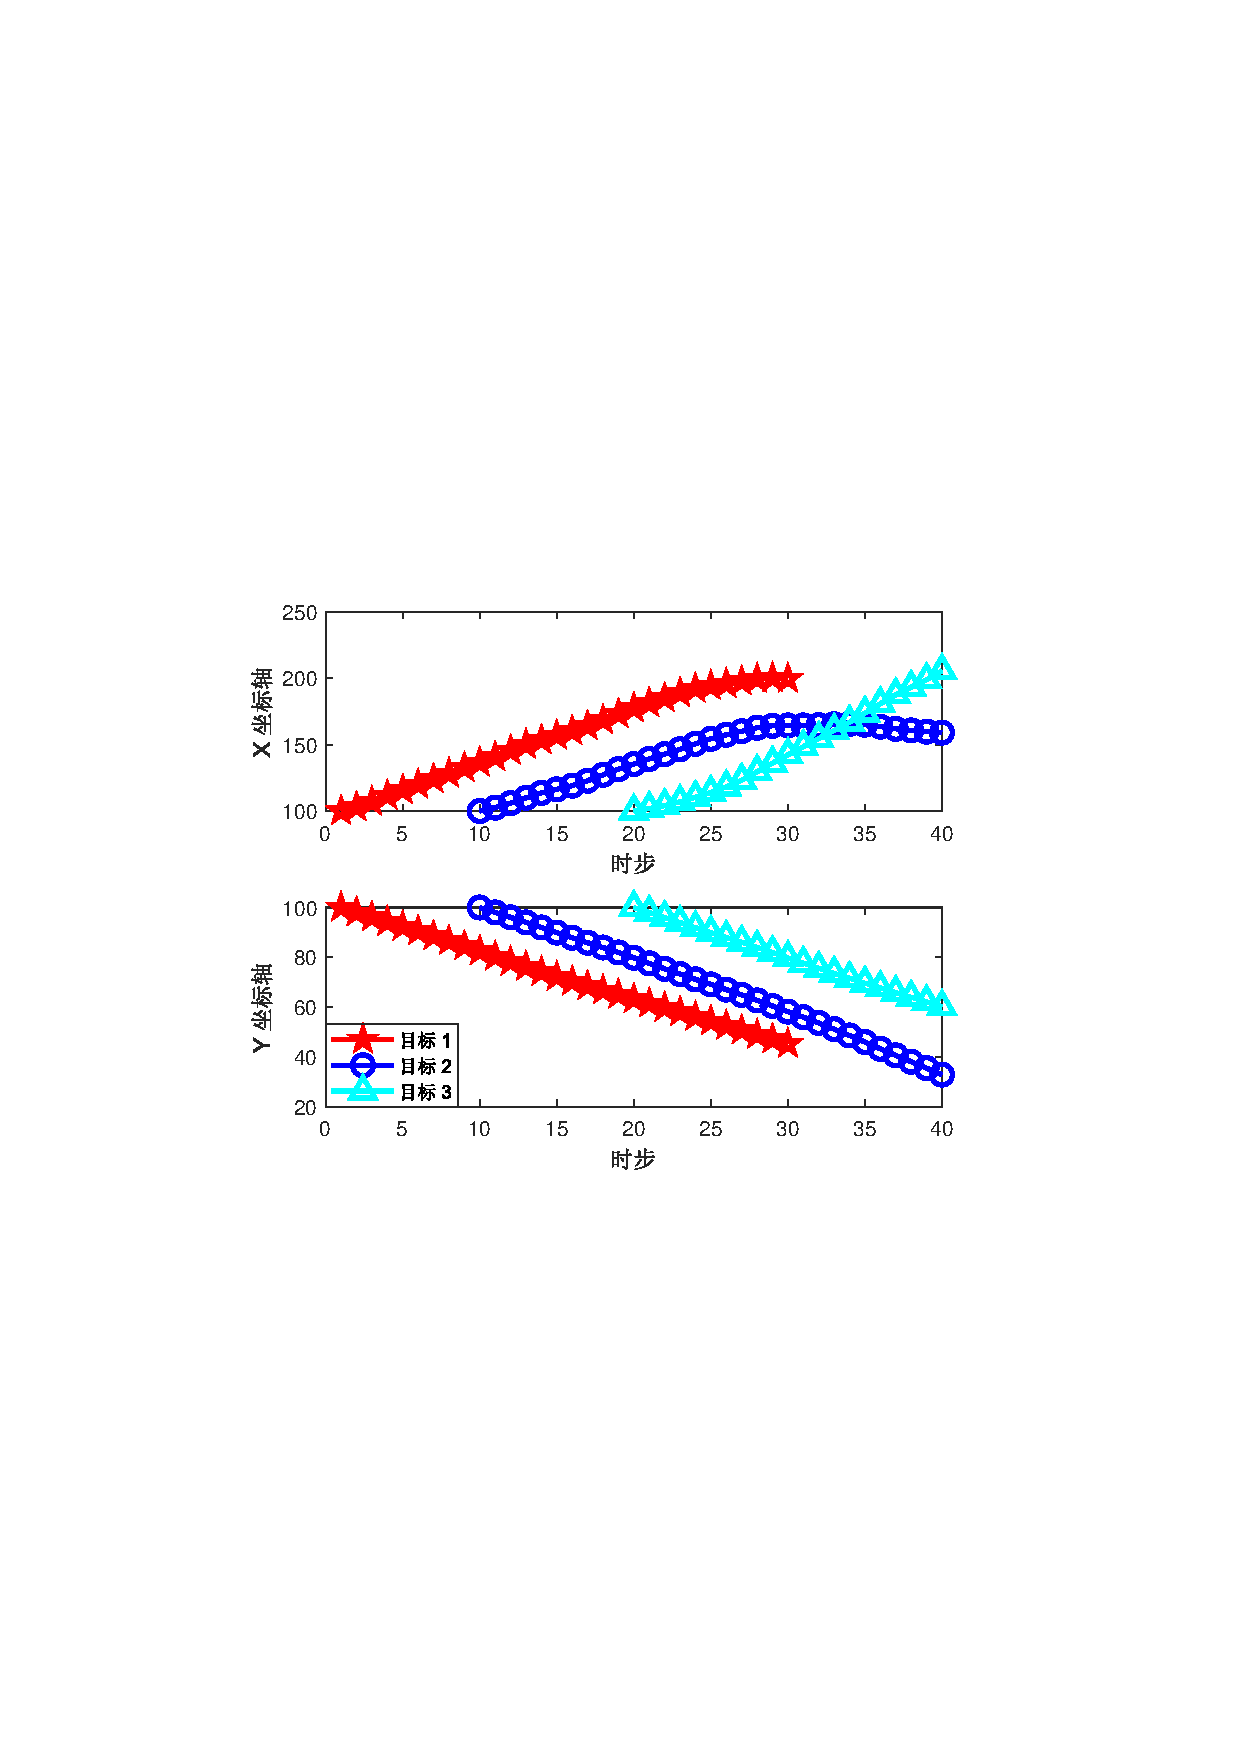
\includegraphics[width=0.7\textwidth]{Pictures/phds1}
	\caption{多个目标在X轴和Y轴上的真实位置}
	\label{fig:06}
\end{figure}
	
\begin{figure}[htbp]
	\centering
	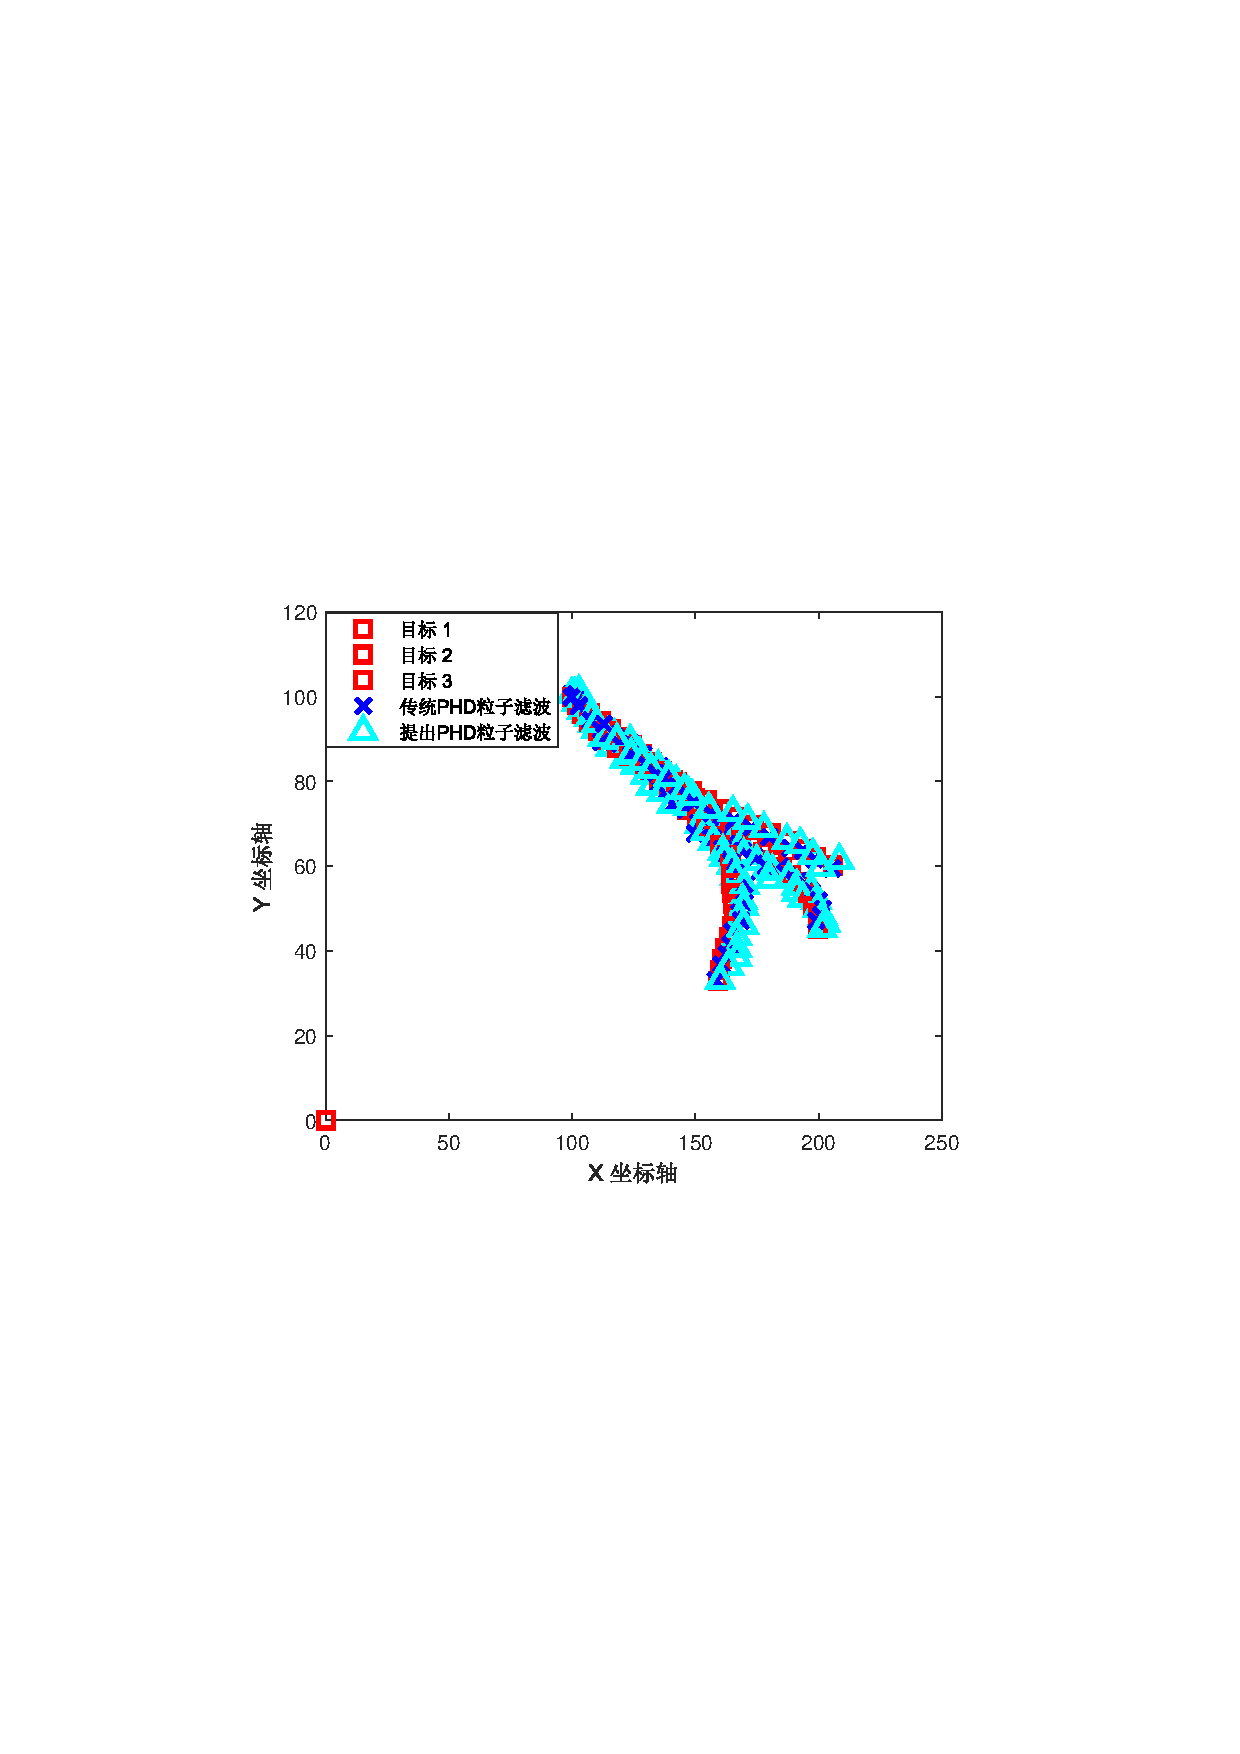
\includegraphics[width=0.7\textwidth]{Pictures/phds2}
	\caption{观测区域内的目标位置与两种PHD滤波算法估计值的比较}
	\label{fig:07}
\end{figure}

此外,图(\ref{fig:09})定量地比较了提出PHD粒子滤波算法与传统粒子滤波算法之间在目标数量估计上的误差。可以看出,两种滤波算法都能够准确地估计出目标的数量,其误差来源可能源于聚类算法。图(\ref{fig:10})使用最优子图分配(Optimal Subpattern Assignment,OSPA)距离\cite{schuhmacher2008consistent} 对跟踪效果进行评价。
OSPA距离是一种基于Wasserstein距离\cite{vallender1974calculation}的多目标误差距离的性能评价指标,同时考虑两个集合之间点位置之间的差距以及集合之间势的差距。具体来说,对于任意有限集合$X=\left\{x_1,\dots,x_m\right\}$与集合$Y\left\{y_1,\dots,y_n\right\}$之间的OSPA距离$\bar{d}^{(c)}_p(X,Y)$表示为
如果$m\leq n$,
\begin{equation}\label{OSPA1}
  \bar{d}^{(c)}_p(X,Y):=\left(\frac{1}{n}\left(\min\limits_{\pi \in \Pi _n}\sum_{i=1}^{m}d^{(c)}(x_i,y_{\pi(i)})^p+c^p(n-m)\right)\right)^{1/p}
\end{equation}

如果$m > n$, $  \bar{d}^{(c)}_p(X,Y):=   \bar{d}^{(c)}_p(Y,X)$。此外,
\begin{equation}\label{OSPA2}
 \bar{d}_{\infty}^{(c)}(X,Y):=\left\{
\begin{aligned}
 & \min\limits_{\pi \in \Pi_n}\max\limits_{1\leq i \leq n}d^{(c)}\left(x_i,y_{\pi(i)}\right) & \text{if} \quad m=n  \\
  & c & \text{if} \quad m\neq n
\end{aligned}\right.
\end{equation}
当$m=n=0$时,$\bar{d}^{(c)}_p(X,Y)=0$。
其中参数$p$为阶数,表示对距离的敏感性。水平参数$c$是截断误差,用以代表对集合势估计的重要性。当$p$增加而$c$不变时,误差距离更加注重估计位置不准确的点;当$c$增加而$p$不变时而,系统会更加注重两个集合之间势的差距,即目标估计数量的差别。当通过调节$p$与$c$的大小,可以避免了Wasserstein距离关于集合之间势差别惩罚过重的缺点。
OSPA中参数$p=2$ , $c=100$取自文献\cite{shi2013threshold}。可以看出两种滤波算法能够相近的跟踪效果。

图(\ref{fig:212})展示了两个算法经过200次蒙特卡洛实验后得到的平均OSPA距离估计误差,可以看到提出的PHD粒子滤波算法与传统PHD粒子滤波算法的跟踪精度都很高,两者没有跟踪性能上的明显差距。

\begin{figure}[htbp]
\centering
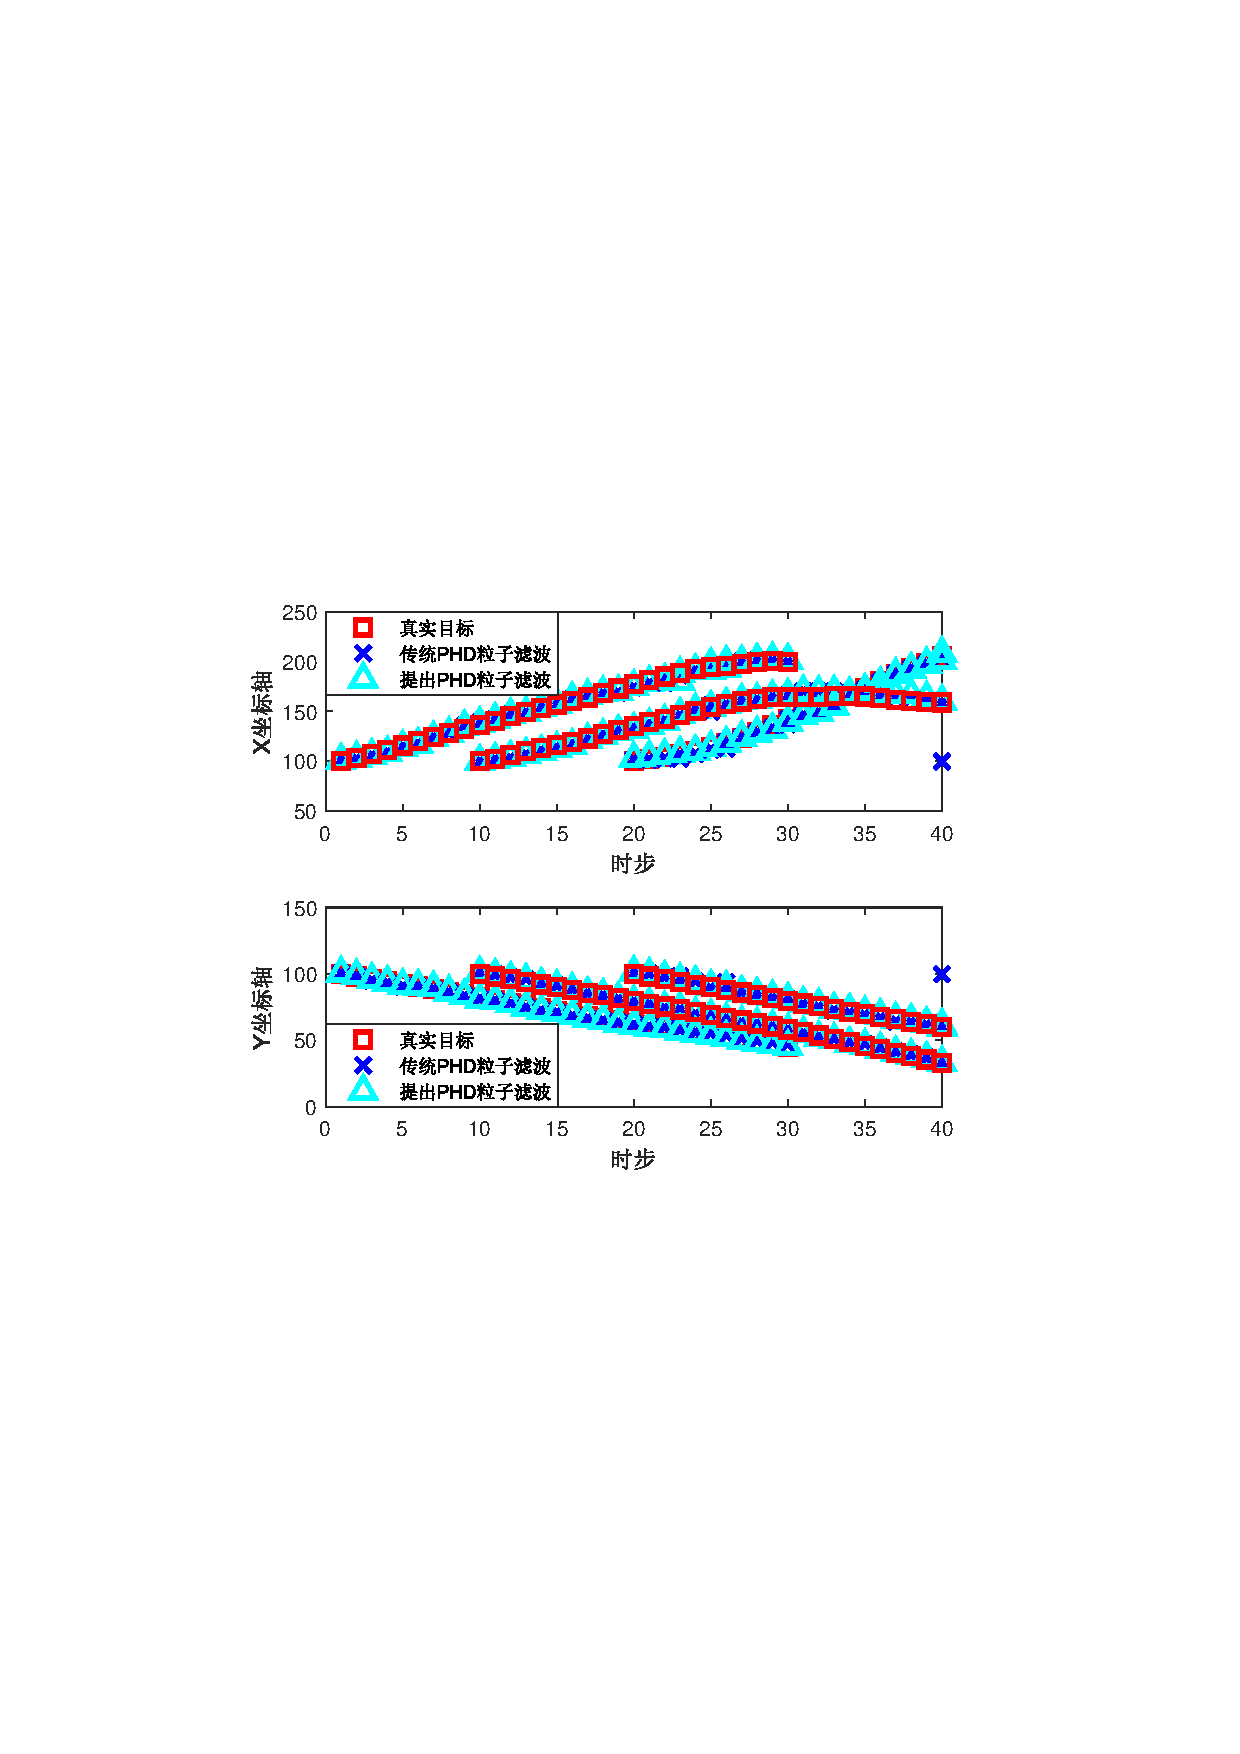
\includegraphics[width=0.7\textwidth]{Pictures/phds3}
\caption{提出的PHD滤波算法与传统PHD滤波算法在位置估计上的比较}
\label{fig:09}
\end{figure}

\begin{figure}[htbp]
\centering
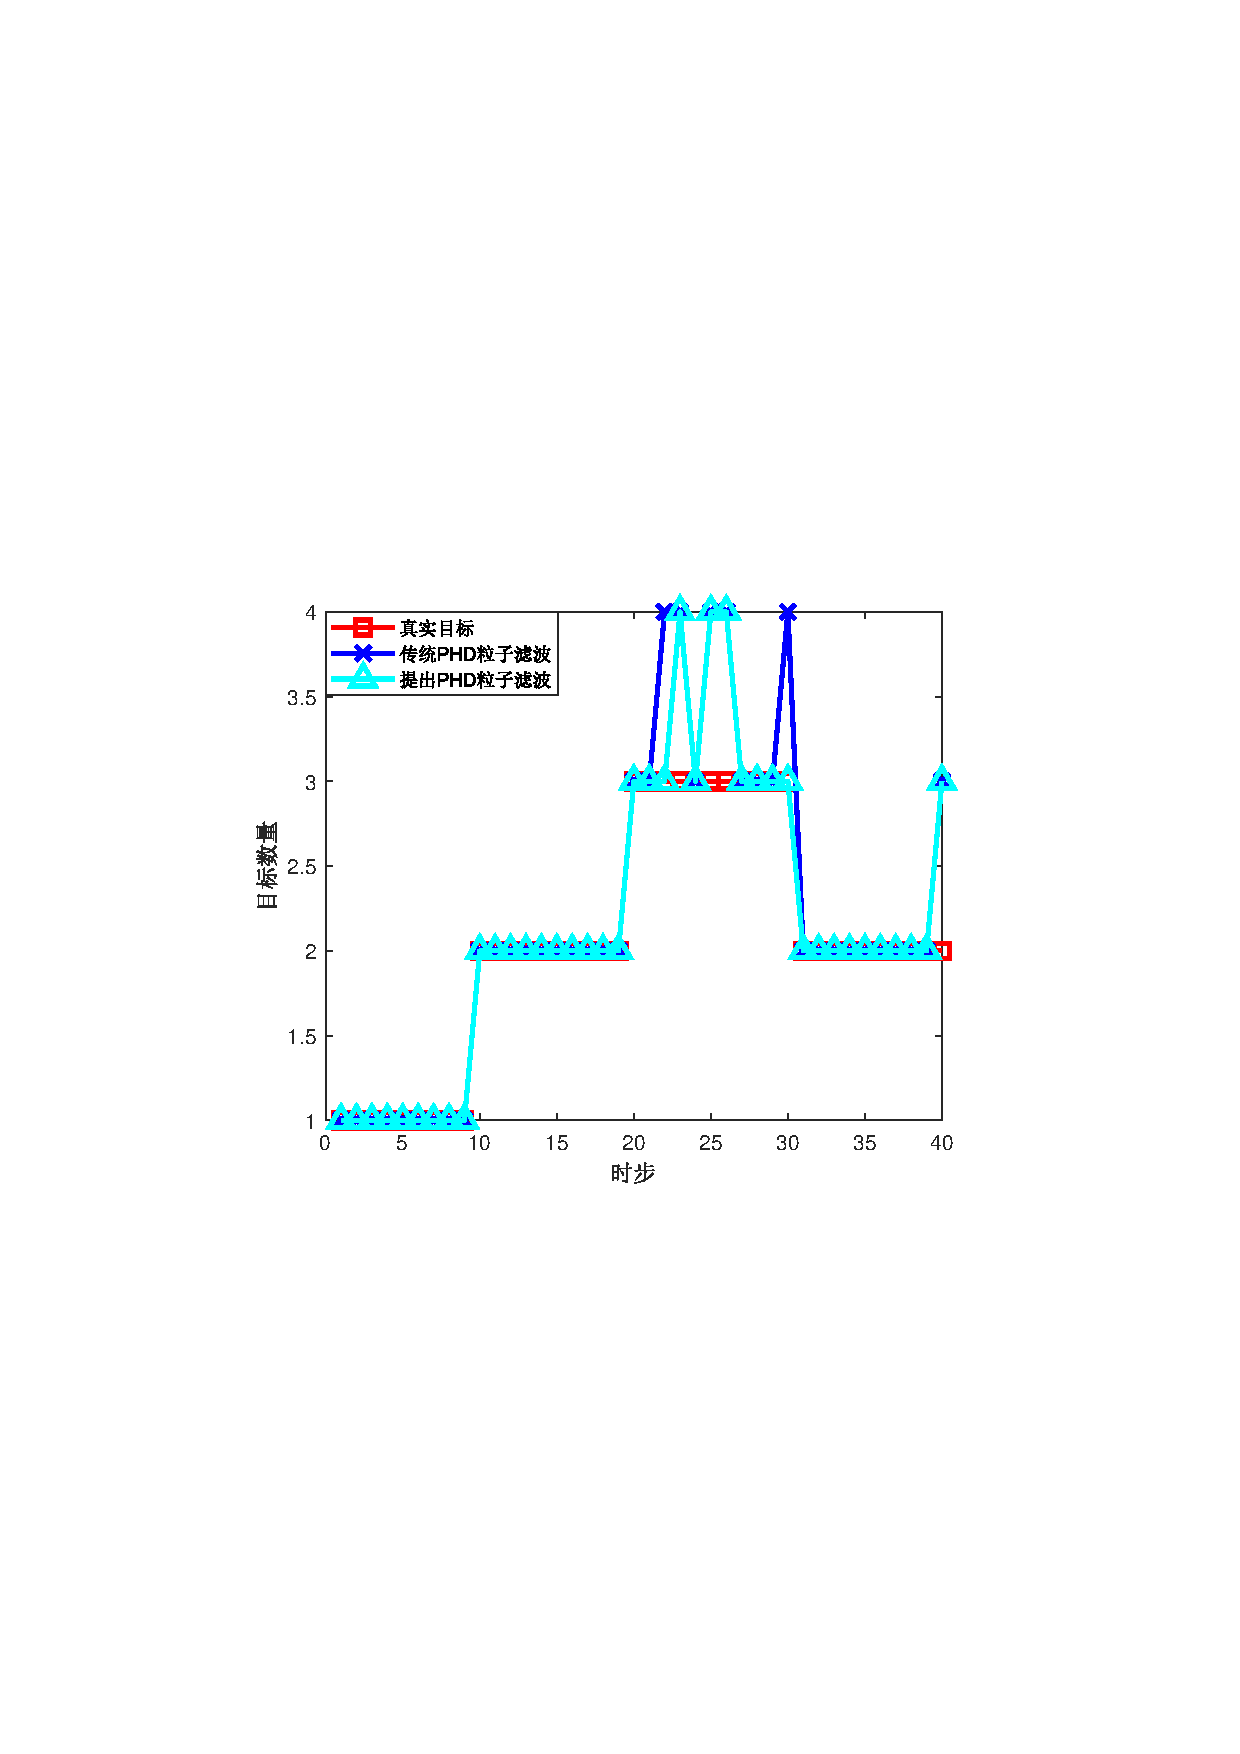
\includegraphics[width=0.7\textwidth]{Pictures/phds5}
\caption{两种PHD滤波算法跟踪目标数量的对比}
\label{fig:10}
\end{figure}

\begin{figure}[htbp]
\centering
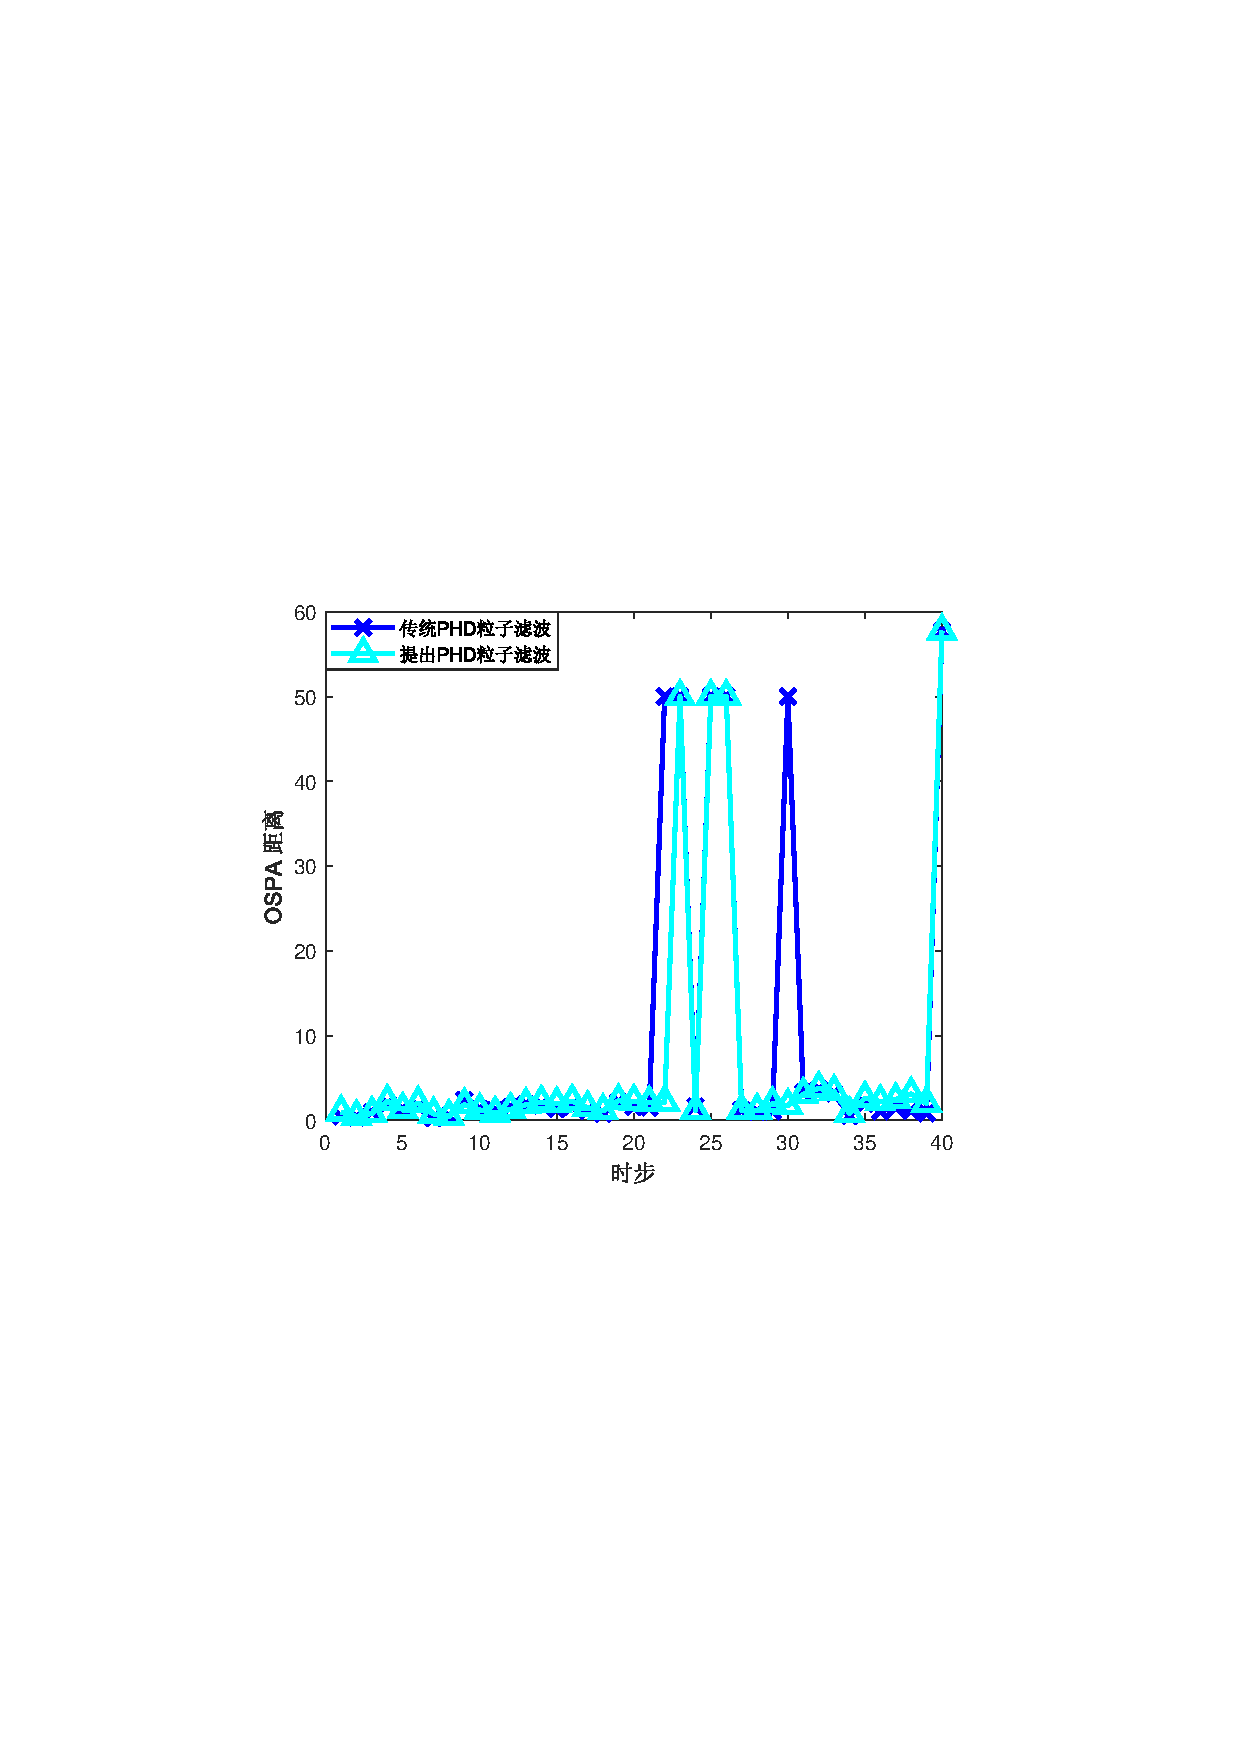
\includegraphics[width=0.7\textwidth]{Pictures/phds4}
\caption{两种PHD滤波算法跟踪效果的OSPA距离的对比}
\label{fig:11}
\end{figure}


\begin{figure}[htbp]
\centering
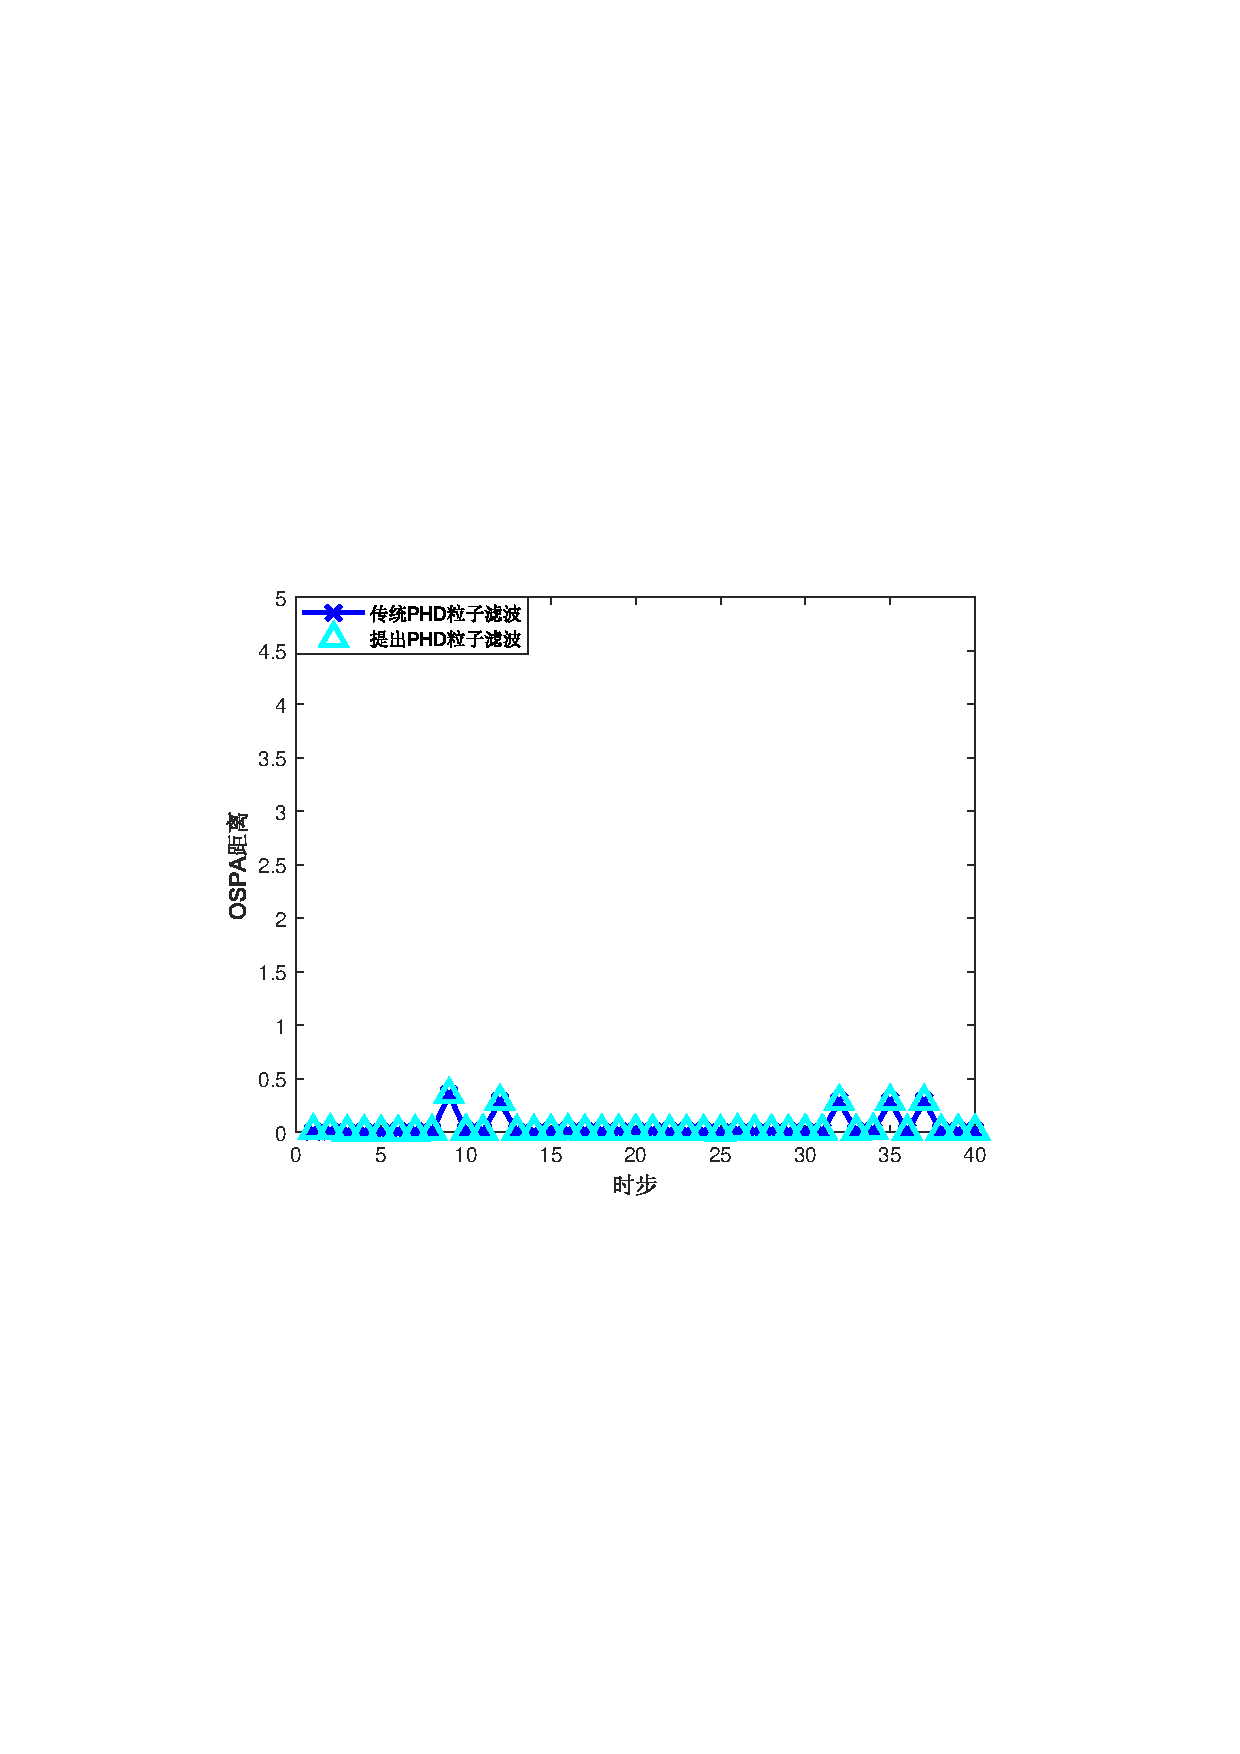
\includegraphics[width=0.7\textwidth]{Pictures/phds6}
\caption{200次Monte Carlo实验后两种PHD算法平均OSPA距离的对比}
\label{fig:212}
\end{figure}

仿真结果显示提出的全流水线全并行PHD粒子滤波算法能够和传统PHD粒子滤波算法达到相同的跟踪水平。

\subsection{时延分析}

图(\ref{fig:08})展示了可用硬件计算资源与总运行时延之间的关系。假设每个滤波算法中的处理器使用一个计算核心。本算法运行在一台使用频率3.2GHz的Intel\textregistered  ~Core\texttrademark ~ i5-4570 CPU上。实验中每个步骤的运行时延分别为$T_{u}=0.357$毫秒, $T_{r}=0.072$毫秒, $T_{p1}=0.041$毫秒, $T_{p2}=0.036$毫秒和 $T_{c}=0.102$毫秒。红色方块代表传统PHD粒子滤波算法,没有使用流水线并行机制和处理器优化的情况,即重采样和预测过程没有流水线化运行,处理器平均配置。则根据运行情况1,总的运行时延可以表示为$T=\begin{aligned}\lceil\frac{L+J}{R_{u}}\rceil T_{u}+\lceil\frac{R_{u}}{R_{r}}\rceil T_{r}+\lceil\frac{L+J}{R_{p1}}\rceil T_{p1}\end{aligned}$。蓝色十字表示的是改进PHD粒子滤波算法只使用改进的重采样算法使得重采样和预测过程可以流水线化运行,而不进行处理器资源优化。则总运行时延可以表示为$T=\begin{aligned}\lceil\frac{L+J}{R_{u}}\rceil T_{u} + \end{aligned} $ $\begin{aligned}   \lceil\frac{R_{u}}{R_{r}}\rceil T_{r}+\lceil\frac{L}{L+J}\frac{R_r}{R_{p1}}\rceil T_{p1}\end{aligned}$。绿色圆圈代表使用改进的PHD粒子滤波算法及处理器资源优化。则总的运行时延为$T=\begin{aligned}\lceil\frac{L+J} {R_{u}}\rceil T_{u}+\lceil\frac{R_{u}}{R_{r}}\rceil T_{r}+\lceil\frac{L}{L+J}\frac{R_r}{R_{p1}}\rceil T_{p1}\end{aligned}$。如图所示,随着处理器数量的增长,总的运行时延在逐步降低。当总的处理器数量固定的时候,提出的完全流水线完全并行化PHD粒子滤波算法结构只需消耗传统滤波算法一半的运行时延,有效地证明了提出算法可以显著提高多目标跟踪的实时性。

\begin{figure}[htbp]
\centering
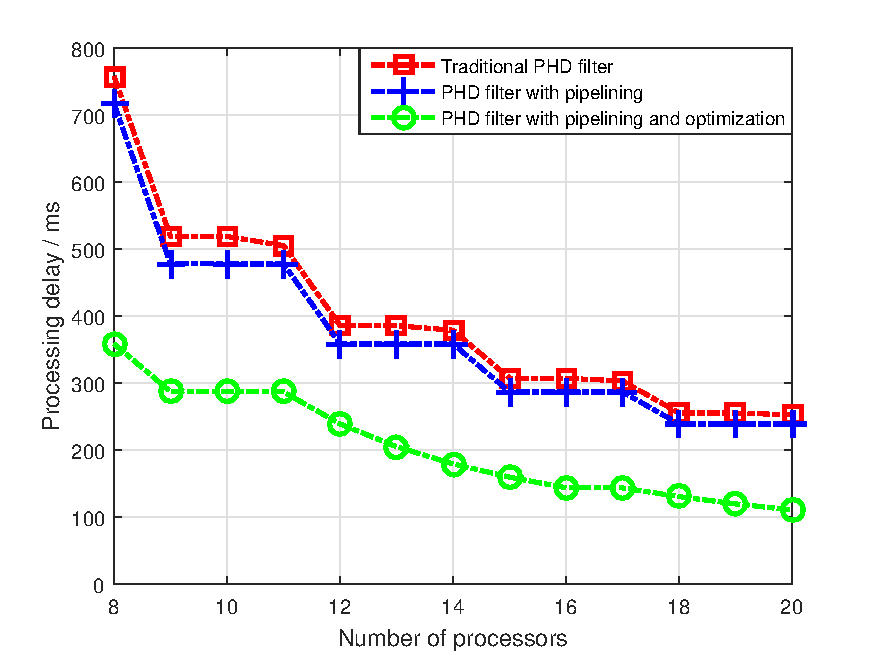
\includegraphics[width=0.7\textwidth]{Pictures/PHD-5}
\caption{不同处理器数量下的运行时延分析}
\label{fig:08}
\end{figure}

\section{本章小结}

在下一代无线通信系统中,基站需要通过毫米波波束同时和多个用户进行方向性通信。为了建立方向性通信并降低通信时延,就需要对这些用户做波束跟踪并实时地得到多用户的位置跟踪信息。本章通过提出一个改进的重采样算法,得到了一个针对多目标跟踪场景的完全流水线完全并行化PHD粒子滤波算法,同时提出了针对多核处理器平台的改进PHD粒子滤波算法及其硬件分配结构。为了提高多目标跟踪的实时性,建立了最小化总运行时延的优化问题并得到了高效的解法。仿真结果表明,相较于传统的PHD粒子滤波算法,提出的完全流水线完全并行化PHD粒子滤波算法大大降低了系统的运行时延,同时保持着相近的跟踪效果。即通过引入改进的重采样算法,提出的优化后算法能够显著提高多目标跟踪的实时性,进而可以降低毫米波无线通信中用户终端的波束对准与跟踪等过程的时延。在实时得到多用户位置及跟踪信息后,下一章将利用这些信息进行小区内多用户通信系统的资源优化分配。
